%!TEX TS-program = xelatex
\documentclass[11pt]{article}

\usepackage[english]{babel}

\usepackage{amsmath,amssymb,amsfonts}
\usepackage[utf8]{inputenc}
\usepackage[T1]{fontenc}
\usepackage{stix}
\usepackage[scaled]{helvet}
\usepackage[scaled]{inconsolata}

\usepackage{lastpage}

\usepackage{setspace}

\usepackage{ccicons}

\usepackage[hang,flushmargin]{footmisc}

\usepackage{geometry}

\setlength{\parindent}{0pt}
\setlength{\parskip}{6pt plus 2pt minus 1pt}

\usepackage{fancyhdr}
\renewcommand{\headrulewidth}{0pt}\providecommand{\tightlist}{%
  \setlength{\itemsep}{0pt}\setlength{\parskip}{0pt}}

\makeatletter
\newcounter{tableno}
\newenvironment{tablenos:no-prefix-table-caption}{
  \caption@ifcompatibility{}{
    \let\oldthetable\thetable
    \let\oldtheHtable\theHtable
    \renewcommand{\thetable}{tableno:\thetableno}
    \renewcommand{\theHtable}{tableno:\thetableno}
    \stepcounter{tableno}
    \captionsetup{labelformat=empty}
  }
}{
  \caption@ifcompatibility{}{
    \captionsetup{labelformat=default}
    \let\thetable\oldthetable
    \let\theHtable\oldtheHtable
    \addtocounter{table}{-1}
  }
}
\makeatother

\usepackage{array}
\newcommand{\PreserveBackslash}[1]{\let\temp=\\#1\let\\=\temp}
\let\PBS=\PreserveBackslash

\usepackage[breaklinks=true]{hyperref}
\hypersetup{colorlinks,%
citecolor=blue,%
filecolor=blue,%
linkcolor=blue,%
urlcolor=blue}
\usepackage{url}

\usepackage{caption}
\setcounter{secnumdepth}{0}
\usepackage{cleveref}

\usepackage{graphicx}
\makeatletter
\def\maxwidth{\ifdim\Gin@nat@width>\linewidth\linewidth
\else\Gin@nat@width\fi}
\makeatother
\let\Oldincludegraphics\includegraphics
\renewcommand{\includegraphics}[1]{\Oldincludegraphics[width=\maxwidth]{#1}}

\usepackage{longtable}
\usepackage{booktabs}

\usepackage{color}
\usepackage{fancyvrb}
\newcommand{\VerbBar}{|}
\newcommand{\VERB}{\Verb[commandchars=\\\{\}]}
\DefineVerbatimEnvironment{Highlighting}{Verbatim}{commandchars=\\\{\}}
% Add ',fontsize=\small' for more characters per line
\usepackage{framed}
\definecolor{shadecolor}{RGB}{248,248,248}
\newenvironment{Shaded}{\begin{snugshade}}{\end{snugshade}}
\newcommand{\KeywordTok}[1]{\textcolor[rgb]{0.13,0.29,0.53}{\textbf{#1}}}
\newcommand{\DataTypeTok}[1]{\textcolor[rgb]{0.13,0.29,0.53}{#1}}
\newcommand{\DecValTok}[1]{\textcolor[rgb]{0.00,0.00,0.81}{#1}}
\newcommand{\BaseNTok}[1]{\textcolor[rgb]{0.00,0.00,0.81}{#1}}
\newcommand{\FloatTok}[1]{\textcolor[rgb]{0.00,0.00,0.81}{#1}}
\newcommand{\ConstantTok}[1]{\textcolor[rgb]{0.00,0.00,0.00}{#1}}
\newcommand{\CharTok}[1]{\textcolor[rgb]{0.31,0.60,0.02}{#1}}
\newcommand{\SpecialCharTok}[1]{\textcolor[rgb]{0.00,0.00,0.00}{#1}}
\newcommand{\StringTok}[1]{\textcolor[rgb]{0.31,0.60,0.02}{#1}}
\newcommand{\VerbatimStringTok}[1]{\textcolor[rgb]{0.31,0.60,0.02}{#1}}
\newcommand{\SpecialStringTok}[1]{\textcolor[rgb]{0.31,0.60,0.02}{#1}}
\newcommand{\ImportTok}[1]{#1}
\newcommand{\CommentTok}[1]{\textcolor[rgb]{0.56,0.35,0.01}{\textit{#1}}}
\newcommand{\DocumentationTok}[1]{\textcolor[rgb]{0.56,0.35,0.01}{\textbf{\textit{#1}}}}
\newcommand{\AnnotationTok}[1]{\textcolor[rgb]{0.56,0.35,0.01}{\textbf{\textit{#1}}}}
\newcommand{\CommentVarTok}[1]{\textcolor[rgb]{0.56,0.35,0.01}{\textbf{\textit{#1}}}}
\newcommand{\OtherTok}[1]{\textcolor[rgb]{0.56,0.35,0.01}{#1}}
\newcommand{\FunctionTok}[1]{\textcolor[rgb]{0.00,0.00,0.00}{#1}}
\newcommand{\VariableTok}[1]{\textcolor[rgb]{0.00,0.00,0.00}{#1}}
\newcommand{\ControlFlowTok}[1]{\textcolor[rgb]{0.13,0.29,0.53}{\textbf{#1}}}
\newcommand{\OperatorTok}[1]{\textcolor[rgb]{0.81,0.36,0.00}{\textbf{#1}}}
\newcommand{\BuiltInTok}[1]{#1}
\newcommand{\ExtensionTok}[1]{#1}
\newcommand{\PreprocessorTok}[1]{\textcolor[rgb]{0.56,0.35,0.01}{\textit{#1}}}
\newcommand{\AttributeTok}[1]{\textcolor[rgb]{0.77,0.63,0.00}{#1}}
\newcommand{\RegionMarkerTok}[1]{#1}
\newcommand{\InformationTok}[1]{\textcolor[rgb]{0.56,0.35,0.01}{\textbf{\textit{#1}}}}
\newcommand{\WarningTok}[1]{\textcolor[rgb]{0.56,0.35,0.01}{\textbf{\textit{#1}}}}
\newcommand{\AlertTok}[1]{\textcolor[rgb]{0.94,0.16,0.16}{#1}}
\newcommand{\ErrorTok}[1]{\textcolor[rgb]{0.64,0.00,0.00}{\textbf{#1}}}
\newcommand{\NormalTok}[1]{#1}

\newlength{\cslhangindent}
\setlength{\cslhangindent}{1.5em}
\newlength{\csllabelwidth}
\setlength{\csllabelwidth}{3em}
\newenvironment{CSLReferences}[3] % #1 hanging-ident, #2 entry spacing
 {% don't indent paragraphs
  \setlength{\parindent}{0pt}
  % turn on hanging indent if param 1 is 1
  \ifodd #1 \everypar{\setlength{\hangindent}{\cslhangindent}}\ignorespaces\fi
  % set entry spacing
  \ifnum #2 > 0
  \setlength{\parskip}{#2\baselineskip}
  \fi
 }%
 {}
\usepackage{calc} % for \widthof, \maxof
\newcommand{\CSLBlock}[1]{#1\hfill\break}
\newcommand{\CSLLeftMargin}[1]{\parbox[t]{\maxof{\widthof{#1}}{\csllabelwidth}}{#1}}
\newcommand{\CSLRightInline}[1]{\parbox[t]{\linewidth}{#1}}
\newcommand{\CSLIndent}[1]{\hspace{\cslhangindent}#1}\geometry{verbose,letterpaper,tmargin=2.5cm,bmargin=2.5cm,lmargin=2.5cm,rmargin=4.5cm}

\usepackage{lineno}
\usepackage[nolists,noheads]{endfloat}

\pagestyle{plain}

\doublespacing

\fancypagestyle{normal}
{
  \fancyhf{}
  \fancyfoot[R]{\footnotesize\sffamily\thepage\ of \pageref*{LastPage}}
}
\begin{document}
\thispagestyle{empty}
{\Large\bfseries\sffamily SVD entropy reveals the high complexity of
ecological networks}
\vskip 5em

%
\href{https://orcid.org/0000-0001-6067-1349}{Tanya\,Strydom}%
%
\,\textsuperscript{1,2}\quad %
\href{https://orcid.org/0000-0002-3454-0633}{Giulio V.\,Dalla Riva}%
%
\,\textsuperscript{3}\quad %
\href{https://orcid.org/0000-0002-0735-5184}{Timothée\,Poisot}%
%
\,\textsuperscript{1,2}

\textsuperscript{1}\,Département de Sciences Biologiques, Université de
Montréal\quad \textsuperscript{2}\,Québec Centre for Biodiversity
Sciences\quad \textsuperscript{3}\,School of Mathematics and Statistics,
University of Canterbury


\textbf{Correspondance to:}\\
Timothée Poisot --- \texttt{timothee.poisot@umontreal.ca}\\

\vfill
This work is released by its authors under a CC-BY 4.0 license\hfill\ccby\\
Last revision: \emph{\today}

\clearpage
\thispagestyle{empty}

\vfill
\textbf{\sffamily Abstract: }Quantifying the complexity of ecological
networks has remained elusive. Primarily, complexity has been defined on
the basis of the structural (or behavioural) complexity of the system.
These definitions ignore the notion of `physical complexity,' which can
measure the amount of information contained in an ecological network,
and how difficult it would be to compress. We present relative rank
deficiency and SVD entropy as measures of `external' and `internal'
complexity respectively. Using bipartite ecological networks, we find
that they all show a very high, almost maximal, physical complexity.
Pollination networks, in particular, are more complex when compared to
other types of interactions. In addition, we find that SVD entropy
relates to other structural measures of complexity (nestedness,
connectance, and spectral radius), but does not inform about the
resilience of a network when using simulated extinction cascades, which
has previously been reported for structural measures of complexity. We
argue that SVD entropy provides a fundamentally more `correct' measure
of network complexity and should be added to the toolkit of descriptors
of ecological networks moving forward.
\vfill

\clearpage
\linenumbers
\pagestyle{normal}

Ecologists have turned to network theory because it offers a powerful
mathematical formalism to embrace the complexity of ecological
communities (Jordi Bascompte and Jordano 2007). Indeed, analysing
ecological systems as networks highlighted how their structure ties into
ecological properties and processes (Proulx, Promislow, and Phillips
2005; Poulin 2010), and there has been a subsequent explosion of
measures that purport to capture elements of network structure, to be
related to the ecology of the system they describe (Delmas et al. 2018).
Since the early days of network ecology, ecological networks have been
called ``complex.'' This sustained interest for the notion of complexity
stems, in part, from the strong ties it has to stability (Landi et al.
2018). As such, many authors have looked for clues, in the network
structure, as to why the networks do not collapse (Borrelli 2015;
Staniczenko, Kopp, and Allesina 2013; Gravel, Massol, and Leibold 2016;
Brose, Williams, and Martinez 2006). Yet decades of theoretical
refinements on the relationship between complexity and stability had a
hard time when rigorously tested on empirical datasets (Jacquet et al.
2016); although ecological networks may be complex, our current measures
of complexity do not translate into predictions about stability.

Surprisingly, \emph{complexity} itself has proven an elusive concept to
define in a rigorous way. It has over time been defined as connectance
(Rozdilsky and Stone 2001), as measures of the diversity of species or
their interactions (Landi et al. 2018), or as a combination of species
richness and trophic diversity (Duffy et al. 2007). In short, network
ecology as a field readily assumes that because we have more information
about a system, or because this system has more components, or simply
because this system can be expressed as a network, it follows that the
system is complex. But such a diversity of definitions, for a concept
that is so central to our quest to understand network stability,
decreases the clarity of what complexity means, and what all of these
alternative definitions do actually capture. This is a common thread in
some measures of ecological network structure, as has been discussed at
length for the various definitions of nestedness (Ulrich, Almeida-Neto,
and Gotelli 2009).

None of the previous definitions of complexity are formally wrong, in
that they do capture an aspect of complexity that ultimately ties to the
behaviour of the system, \emph{i.e.} its low predictability over time.
Yet Adami (2002) provides a compelling argument for why the complexity
of the behaviour does not necessarily reflects the complexity of the
system; in fact, one would be very hard pressed to think of a more
simple system than the logistic map used by May (1976) to illustrate how
easily complexity of behaviour emerges. Rather than yielding to the easy
assumption that a system will be complex because it has many parts, or
because it exhibits a complex behaviour, Adami (2002) suggests that we
focus on measuring ``physical complexity,'' \emph{i.e.} the amount of
information required to encode the system, and how much signal this
information contains. Complex systems, in this perspective, are those
who cannot easily be compressed - and this is a notion we can explore
for the structure of ecological networks.

Ecological networks are primarily represented by their adjacency
matrices, \emph{i.e.} a matrix in which every entry represents a pair of
species, which can take a value of 1 when the two species interact, and
a value of 0 when they do not. These matrices (as any matrices) can
easily be factorised using Singular Value Decomposition (Forsythe and
Moler 1967; Gene H. Golub and Reinsch 1971), which offers two
interesting candidate measures of complexity for ecological networks
(both of which we describe at length in the methods). The first measure
is the rank of the matrix, which works as an estimate of ``external
complexity,'' in that it describes the dimension of the vector space of
this matrix, and therefore the number of linearly independent rows (or
columns) of it. From an ecological standpoint, this quantifies the
number of unique ``strategies'' represented in the network: a network
with two modules that are distinct complete graphs has a rank of 2. The
second measure is an application of the entropy measure of Shannon
(1948) to the non-zero singular values of the matrix obtained through
SVD. This so-called SVD entropy measures the extent to which each rank
encodes an equal amount of information, as the singular values capture
the importance of each rank to reconstruct the original matrix; this
approach therefore serves as a measure of ``internal complexity.''

In this manuscript, we present and evaluate the use of both the rank and
SVD entropy of ecological networks as alternative and more robust
measures of complexity when compared to traditional approaches to
defining complexity. This is done by using a collection of 220 bipartite
networks from various types of interaction, sizes, connectances, and
environments. We show that while the rank of the adjacency matrix holds
little information, SVD entropy functions as an appropriate
quantification of the complexity of ecological systems. Notably, SVD
entropy is an intuitive, robust, non-structural approach to defining the
(surprisingly high) complexity of ecological networks, by relating them
to their `physical' as opposed to `behavioural' complexity. In this
process we showcase a breakdown in the assumption that all measures of
complexity of networks are indicative of their robustness to
extinctions. Finally, we show that, despite their high complexity,
observed networks are less complex when compared to pseudo-random
networks, especially for larger networks. We propose that taking a
physical approach to quantifying the complexity of ecological networks
is a step in the right direction to unifying how we define complexity in
the context of ecological networks, as it restores other measures (like
connectance and nestedness) to their original role and signification.

\hypertarget{data-and-methods}{%
\section{Data and methods}\label{data-and-methods}}

We used all bipartite networks contained in the \texttt{web-of-life.es}
database. This database extracted species interaction networks from
supplementary materials across all inhabited continents and covers a
large array of sampling years, environments, organisms, and sampling
methodologies. As such, this dataset is particularly suited to describe
general trends across \emph{all} ecological networks. We specifically
worked on the version of this dataset distributed with the
\texttt{EcologicalNetworks.jl} package (Poisot et al. 2019) for the
\emph{Julia} (Bezanson et al. 2017) programming language, in which all
analyses were conducted. Using bipartite networks means that interacting
species are split into two sets (or interacting groups) and along
different dimensions in the interaction matrix. Thus, columns in the
matrix represent one group (or type) of species and rows represent the
other group of species involved in the interaction. Because SVD gives
similar results on the matrix and its transpose, it captures the
complexity of both sides of the system at once. A summary of the dataset
is given in tbl.~\ref{tbl:summary}.

\hypertarget{tbl:summary}{}
\begin{longtable}[]{@{}lllll@{}}
\caption{\label{tbl:summary}Overview of the \texttt{web-of-life.es}
dataset. We used all networks with up to 500 species. Although there are
spatial biases in the sampling of interaction types (and some
interaction types being under-represented), this dataset covers a range
of latitudes from -43 degrees south to 81 degrees north. The average
richess of the top and bottom level of the bipartite networks are also
given in the last columns.}\tabularnewline
\toprule
Interaction type & Sample size & Latitude range & Richness (top) &
Richness (bottom)\tabularnewline
\midrule
\endfirsthead
\toprule
Interaction type & Sample size & Latitude range & Richness (top) &
Richness (bottom)\tabularnewline
\midrule
\endhead
Host-Parasite & 51 & 38.77 \(\rightarrow\) 72.65 & 20.47 &
12.23\tabularnewline
Plant-Ant & 4 & -16.11 \(\rightarrow\) -2.40 & 18.75 &
21.75\tabularnewline
Plant-Herbivore & 4 & 30.20 \(\rightarrow\) 64.91 & 49.5 &
29.25\tabularnewline
Pollination & 134 & -43.09 \(\rightarrow\) 81.81 & 40.22 &
18.02\tabularnewline
Seed Dispersal & 33 & -28.95 \(\rightarrow\) 53.05 & 18.75 &
25.12\tabularnewline
\bottomrule
\end{longtable}

\hypertarget{estimating-complexity-with-rank-deficiency}{%
\subsection{Estimating complexity with rank
deficiency}\label{estimating-complexity-with-rank-deficiency}}

The rank of \(\mathbf{A}\) (noted as \(r = \text{rk}(\mathbf{A})\)) is
the dimension of the vector space spanned by the matrix and corresponds
to the number of linearly independent rows or columns; therefore, the
maximum rank of a matrix (\(M = \text{rk}_{\text{max}}(\mathbf{A})\))
will always be equal to the length of the shortest dimension of
\(\mathbf{A}\), which ecologically speaking is the richness of the least
species-rich compartment of the bipartite network (or the richness in
the case of unipartite networks). A matrix is ``full-ranked'' when
\(r=M\), \emph{i.e.} all of its rows/columns are unique. Matrices that
are not full-ranked are called rank deficient, and we can measure rank
deficiency using \(d = M-r\). So as to control for the difference in
species richness of the different networks, we report the relative rank
deficiency, \emph{i.e.} expressed as a ratio between rank deficiency and
the maximal rank:

\begin{equation}\protect\hypertarget{eq:rankdeficiency}{}{D = 1-\frac{r}{M}}\label{eq:rankdeficiency}\end{equation}

This measure returns values between 0 (the matrix is full ranked) and
\(1-M^{-1} \approx 1\) (the matrix has rank 1). This serves as a coarse
estimate of complexity, as the more unique columns/rows are in the
matrix, the larger this value will be. Yet it may also lack sensitivity,
because it imposes a stringent test on uniqueness, which calls for more
quantitative approaches to complexity.

\hypertarget{estimating-complexity-with-svd-entropy}{%
\subsection{Estimating complexity with SVD
entropy}\label{estimating-complexity-with-svd-entropy}}

Singular Value Decomposition (SVD) is the factorisation of a matrix
\(\mathbf{A}\) (where \(\mathbf{A}_{m,n} \in\mathbb{B}\) in our case,
but SVD works for matrices of real numbers as well) into the form
\(\mathbf{U}\cdot\mathbf{\Sigma}\cdot \mathbf{V}^T\). Where
\(\mathbf{U}\) is an \(m \times m\) orthogonal matrix and \(\mathbf{V}\)
an \(n \times n\) orthogonal matrix. The columns in these matrices are,
respectively, the left- and right-singular vectors of \(\mathbf{A}\),
were \(\mathbf{U} = \mathbf{A}\mathbf{A}^T\) and
\(\mathbf{V} = \mathbf{A}^T\mathbf{A}\). \(\mathbf{\Sigma}\) is a matrix
that only contains non-negative \(\sigma\) values along its diagonal and
all other entries are zero. Where \(\sigma_{i} = \Sigma{ii}\), which
contains the singular values of \(\mathbf{A}\). When the values of
\(\mathbf{\sigma}\) are arranged in descending order, the singular
values (\(\mathbf{\Sigma}\)) are unique, though the singular vectors
(\(\mathbf{U}\) and \(\mathbf{V}\)) may not be.

After the Eckart-Young-Mirsky theorem (Eckart and Young 1936; G. H.
Golub, Hoffman, and Stewart 1987), the number of non-zero entries (after
rounding of small values if required due to numerical precision issues
in computing the factorisation) in \(\mathbf{\sigma}\) is the rank of
matrix \(\mathbf{A}\). For the sake of simplicity in notation, we will
use \(k = \text{rk}(\mathbf{A})\)) for the rank of the matrix. Because
only the first \(k\) elements of \(\mathbf{\sigma}\) are non-zero, and
that the result of the SVD is a simple matrix multiplication, one can
define a truncated SVD containing only the first \(k\) singular values.

Intuitively, the singular value \(i\) (\(\sigma_i\)) measures how much
of the dataset is (proportionally) explained by each vector - therefore,
one can measure the entropy of \(\mathbf{\sigma}\) following Shannon
(1948). High values of SVD entropy reflects that all vectors are equally
important, \emph{i.e.} that the structure of the ecological network
cannot efficiently be compressed, and therefore indicates high
complexity (Gu and Shao 2016). Because networks have different
dimensions, we use Pielou's evenness (Pielou 1975) to ensure that values
are lower than unity, and quantify SVD entropy, using
\(s_i = \sigma_i/\text{sum}(\sigma)\) as:

\begin{equation}\protect\hypertarget{eq:svdentropy}{}{J = -\frac{1}{\ln(k)}\sum_{i=1}^k s_i\cdot\ln(s_i)}\label{eq:svdentropy}\end{equation}

\hypertarget{results-and-discussion}{%
\section{Results and discussion}\label{results-and-discussion}}

\hypertarget{most-ecological-networks-are-close-to-full-rank}{%
\subsection{Most ecological networks are close to
full-rank}\label{most-ecological-networks-are-close-to-full-rank}}

The majority (63\% of our dataset) of bipartite ecological networks have
a relative rank deficiency of 0 (fig.~\ref{fig:size}), which indicates
that all species have different and unique interaction lists.
Interestingly, the networks that had a comparatively larger relative
rank deficiency tended to be smaller ones. Yet because most of the
networks return the same value, matrix rank does not appear to be a
useful or discriminant measure of network complexity. Another striking
result (from fig.~\ref{fig:size}) is that the SVD entropy of ecological
networks is really large -- although the value can range from 0 to 1,
all ecological networks had SVD entropy larger than 0.8, which is
indicative of a strong complexity.

\begin{figure}
\hypertarget{fig:size}{%
\centering
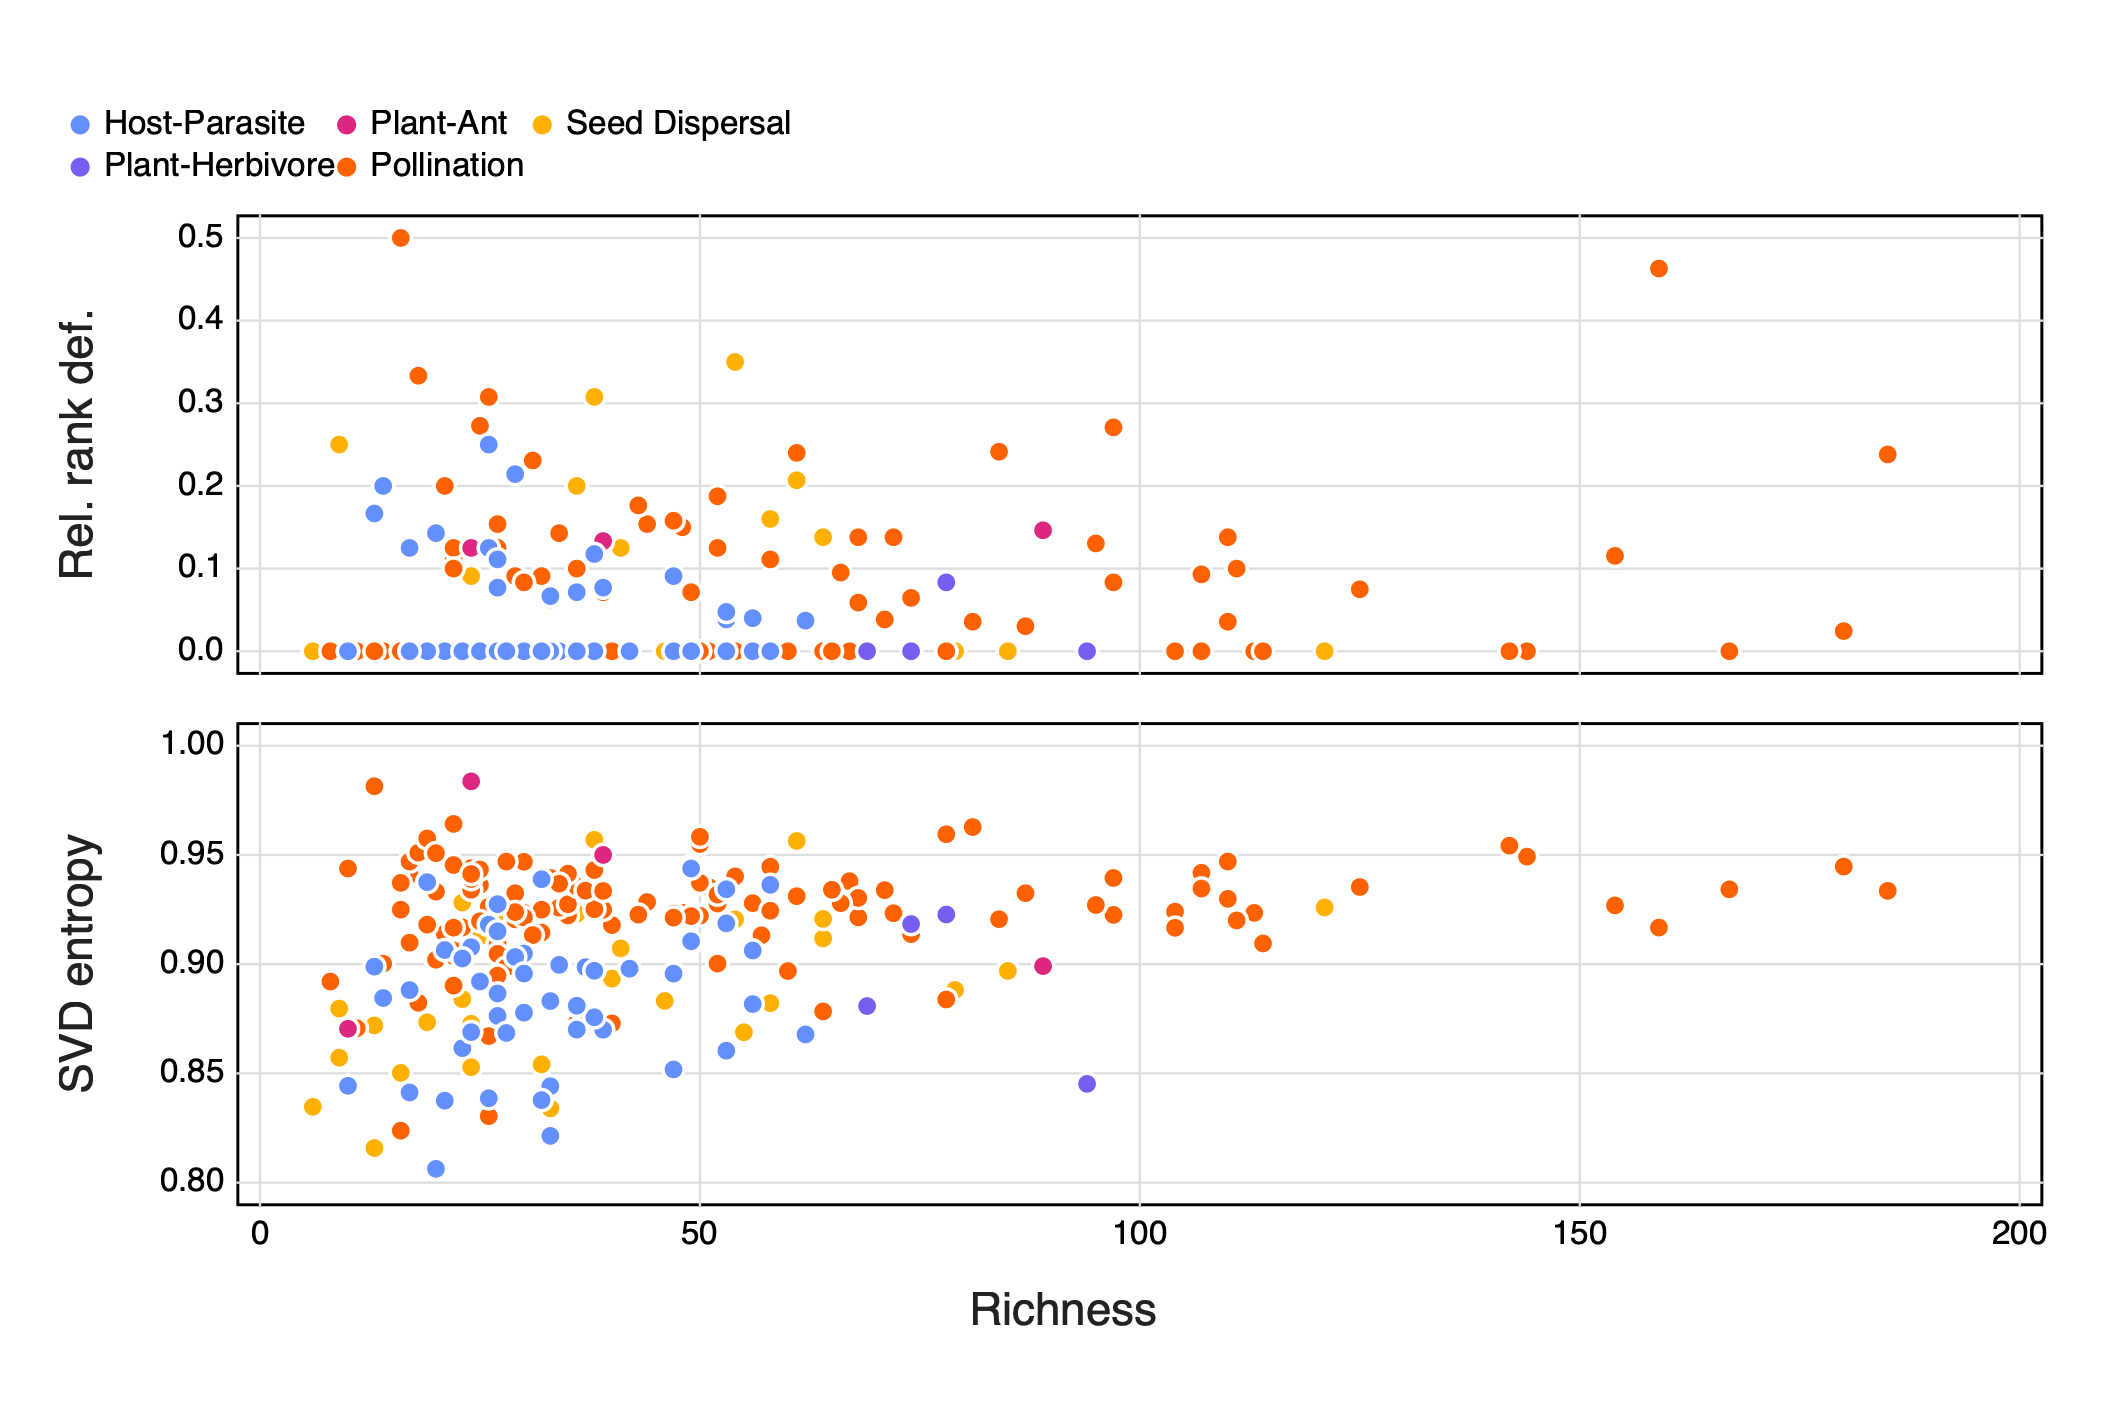
\includegraphics{figures/size_v_rankentropy.png}
\caption{The relationship between network richness and relative rank
deficiency, and SVD entropy. The different types of interactions are
indicated by the colours.}\label{fig:size}
}
\end{figure}

As expected following the observation that ecological networks are
overwhelmingly full ranked, we do not see a relationship between SVD
entropy and relative rank deficiency, neither do we observe differences
between interaction types (fig.~\ref{fig:entropy_v_rank}). Based on
these results, we feel confident that SVD entropy provides a more
informative measure of the complexity of ecological networks, and will
use it moving forward.

\begin{figure}
\hypertarget{fig:entropy_v_rank}{%
\centering
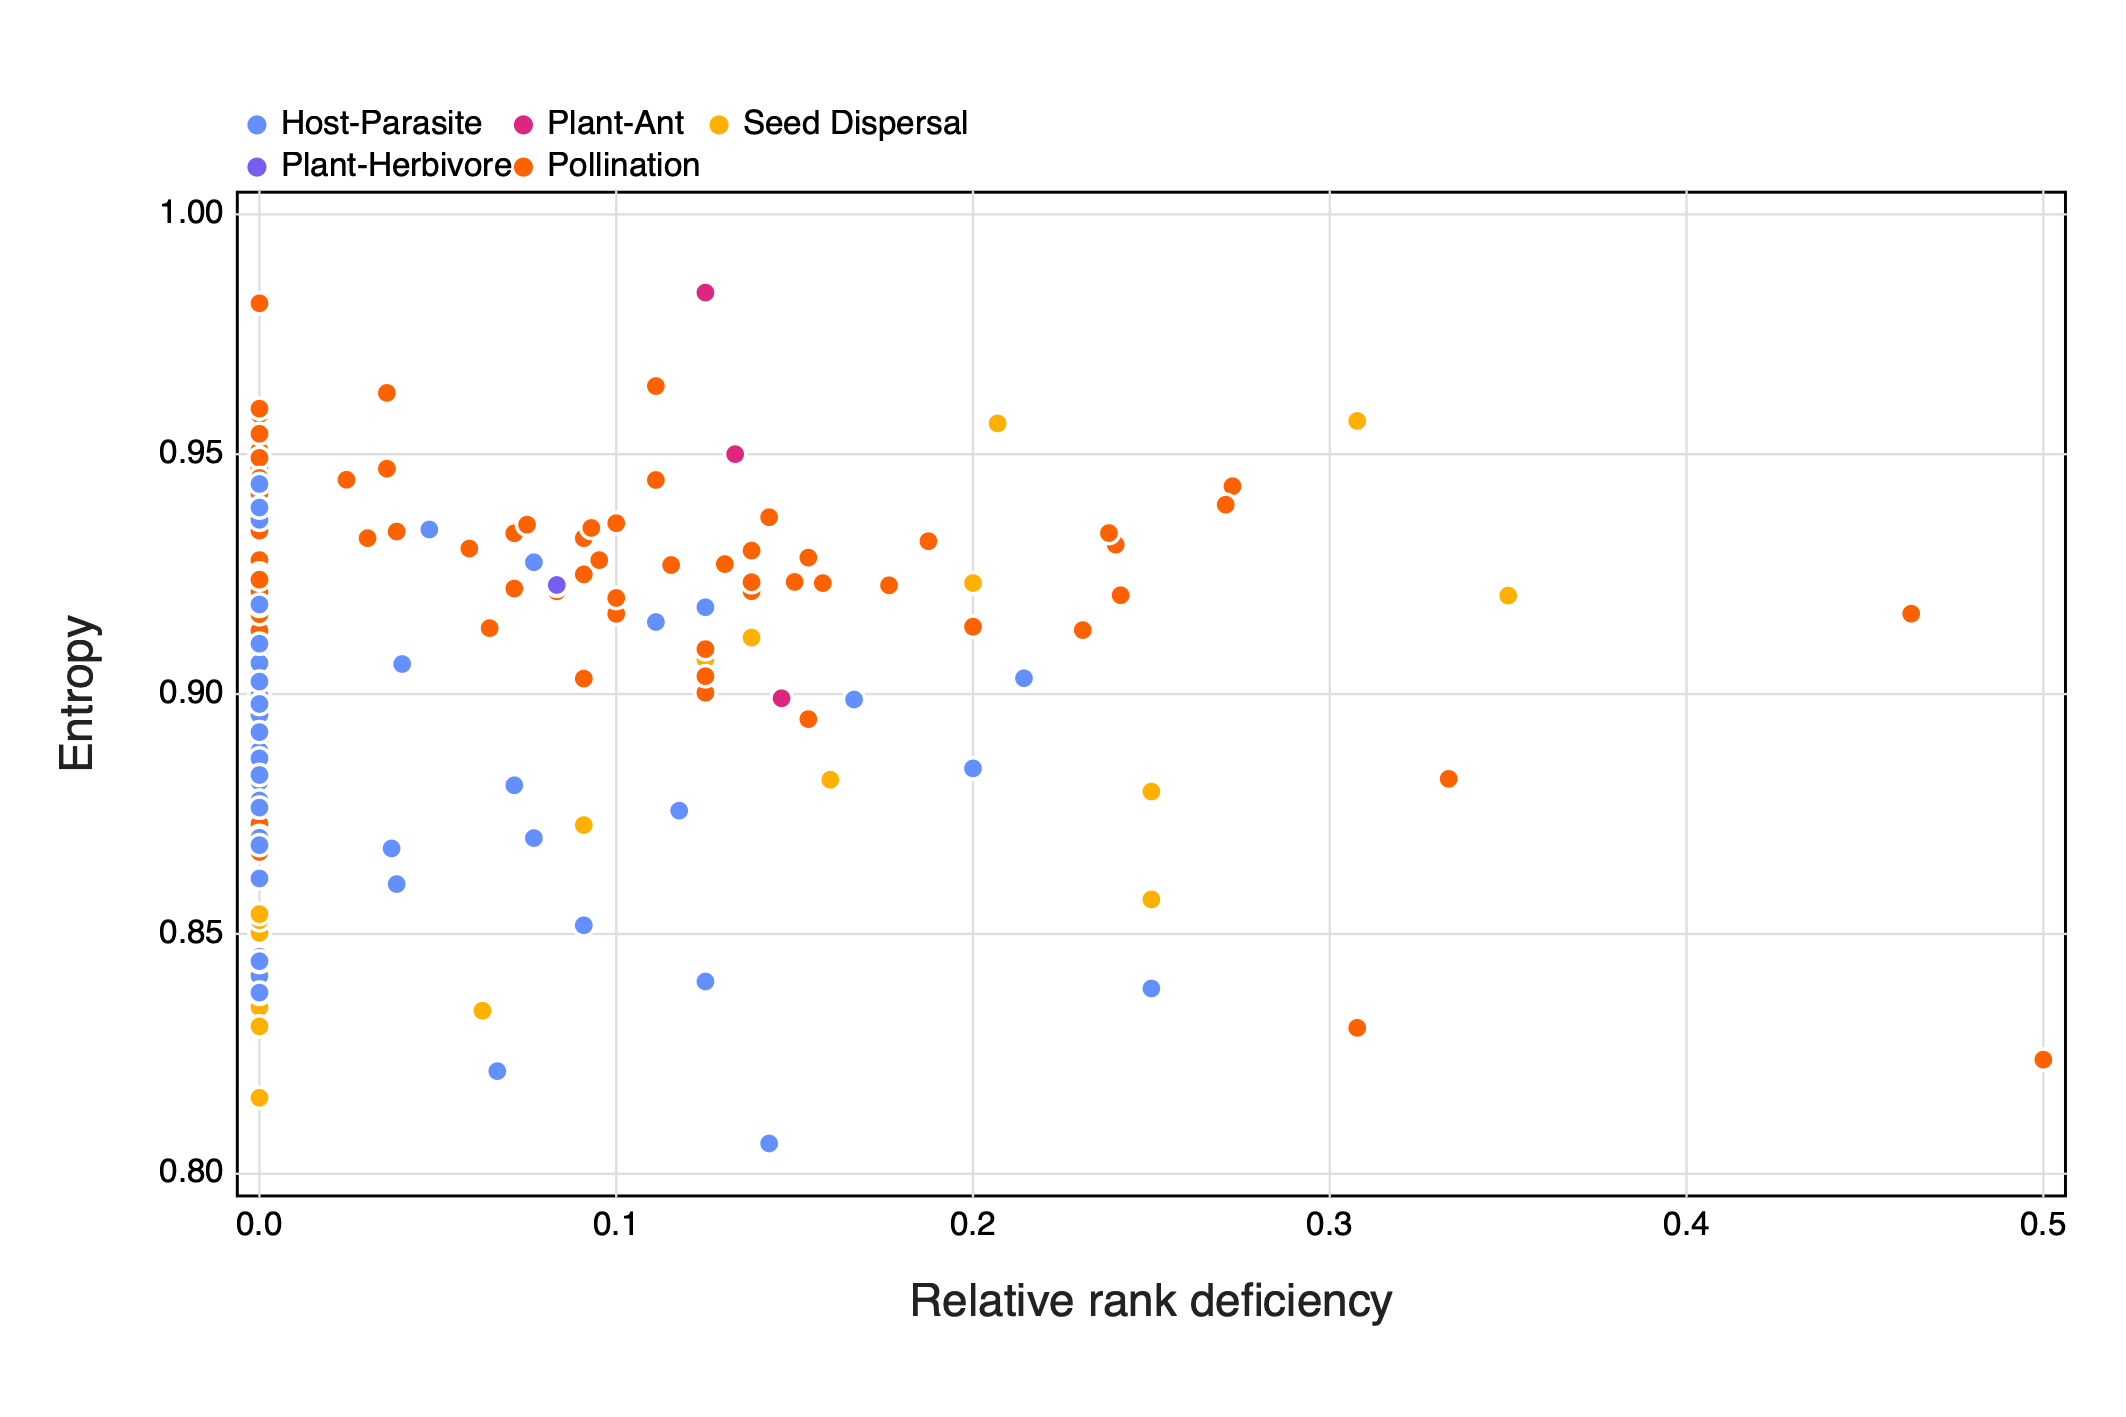
\includegraphics{figures/entropy_v_rank.png}
\caption{The relationship between SVD entropy and the relative rank
deficiency of different species interaction networks Colours indicate
the different interaction types of the
networks.}\label{fig:entropy_v_rank}
}
\end{figure}

\hypertarget{most-elements-of-network-structure-capture-network-complexity}{%
\subsection{Most elements of network structure capture network
complexity}\label{most-elements-of-network-structure-capture-network-complexity}}

We compared SVD entropy to some of the more common measures of
complexity, namely nestedness (\(\eta\), as per Bastolla et al. (2009)),
connectance (\(\text{Co}\)), and the spectral radius of the network
(\(\rho\), following Staniczenko, Kopp, and Allesina (2013)). All of
these measures are positively correlated, especially over the range of
connectances covered by empirical bipartite ecological networks.

Nestedness is calculated based on the number of interactions shared
between species pairs and is a measure of the degree of overlap between
species links (or strategies) in the community, where larger assemblages
are made up of a subset of smaller ones that share common interactions.
Networks with a higher degree of nestedness could be considered simpler
when compared to networks with a lower degree of nestedness. Connectance
is the realised number of interactions (links) in an ecological network
and is calculated as the fraction of the total number of realised
interactions (or links) and the maximum number of possible interactions
in a network (Martinez 1992). This has been shown to be a good estimate
of a community's resilience to perturbation (Dunne, Williams, and
Martinez 2002). The spectral radius of a matrix is the largest absolute
value of its eigenvalues, which, in addition to being presented as a
measure of network complexity has also been suggested as an indicator of
the ability of a system to dampen disturbances (Phillips 2011).

We find that SVD entropy has a clear negative relationship with
nestedness, spectral radius, and connectance (fig.~\ref{fig:other}). As
in fig.~\ref{fig:type}, mutualistic networks tend to be more complex,
and they also are both sparser and less nested than other types of
networks. Bastolla et al. (2009) give a convincing demonstration that
mutualistic networks are shaped to minimise competition -- this can be
done by avoiding to duplicate overlap in interactions, thereby resulting
in a network that is close to full rank, and with high SVD entropy.
Interestingly, fig.~\ref{fig:other} suggests that both nestedness and
connectance measure the \emph{lack} of complexity in an ecological
network, which contrasts to how they may commonly be viewed (Landi et
al. 2018).

\begin{figure}
\hypertarget{fig:other}{%
\centering
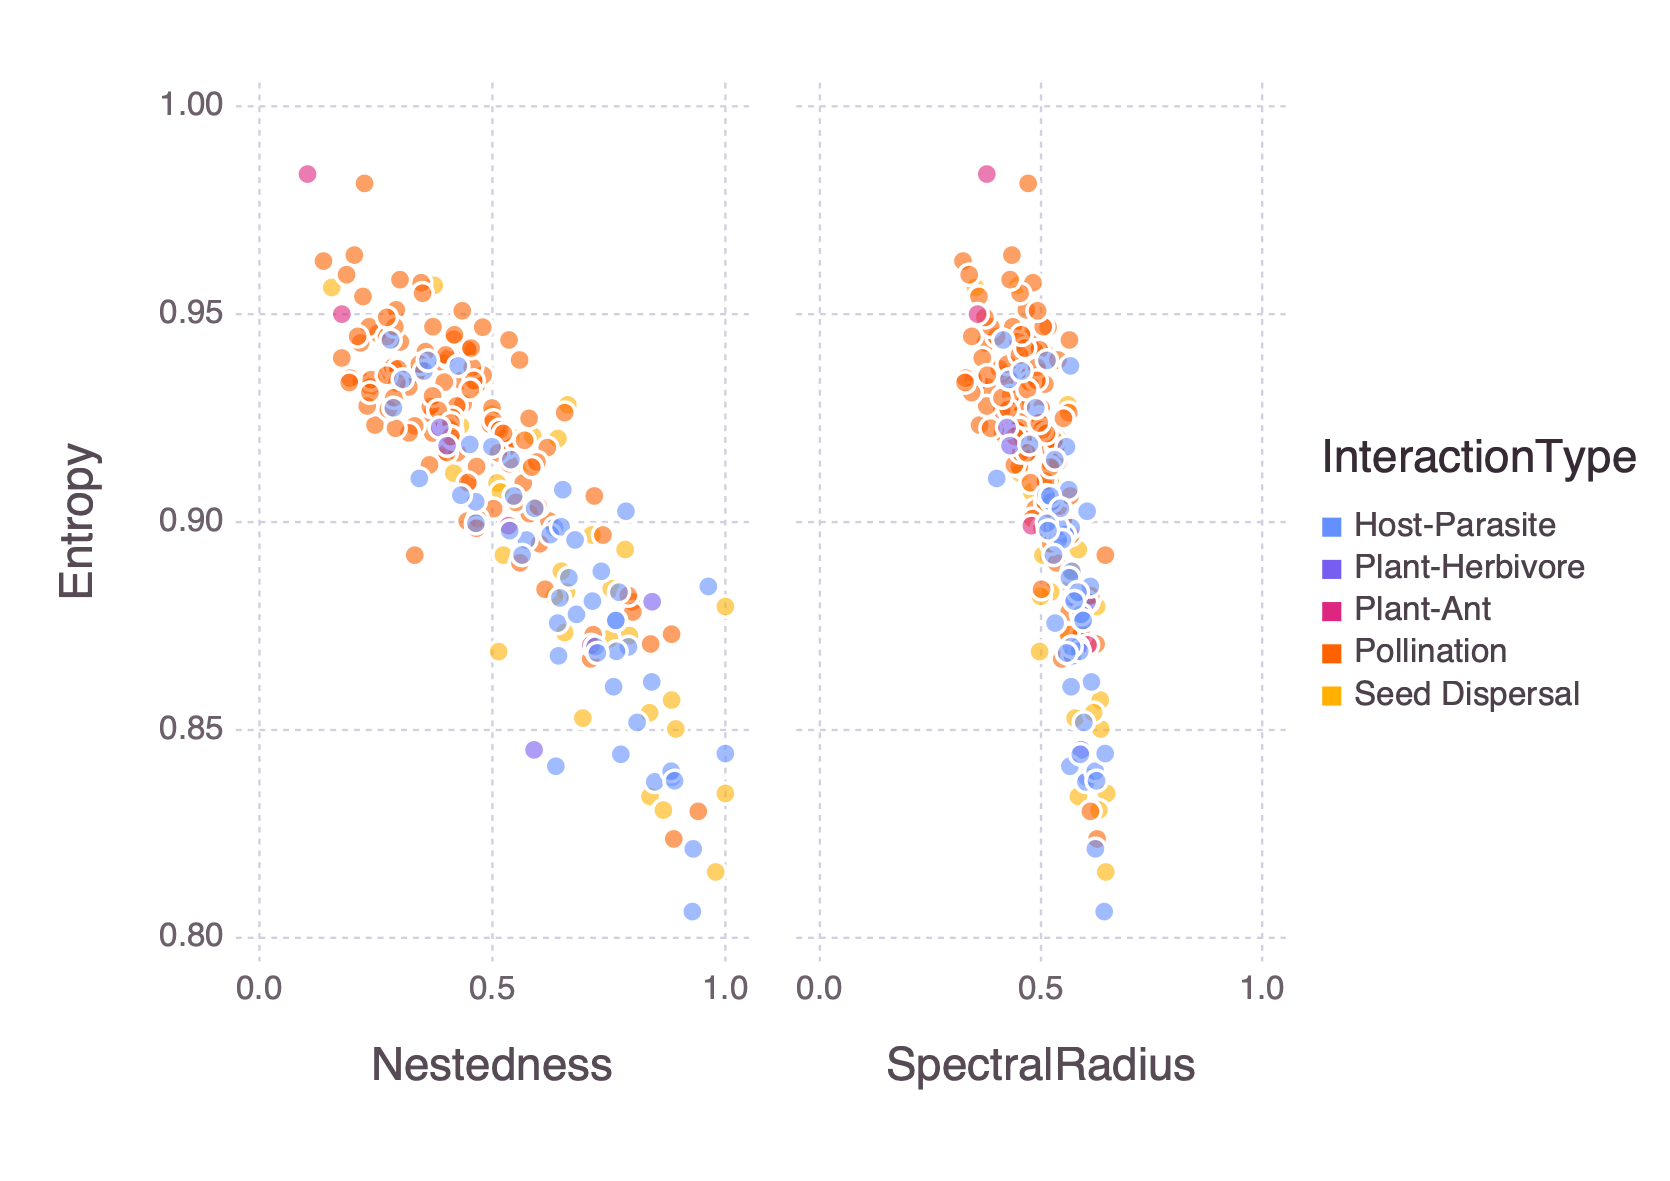
\includegraphics{figures/others_v_entropy.png}
\caption{The relationship between SVD entropy and the nestedness (left
panel), spectral radius (central panel) and connectance (right panel) of
ecological networks. Colours indicate the different interaction types of
the networks.}\label{fig:other}
}
\end{figure}

\hypertarget{complex-networks-are-not-more-robust-to-extinction}{%
\subsection{Complex networks are not more robust to
extinction}\label{complex-networks-are-not-more-robust-to-extinction}}

One approach to calculating the overall structural robustness of an
ecological network is by simulating extinction events through the
sequential removal of species, which allows constructing an extinction
curve that plots the relationship between species removed and cumulative
secondary extinctions (Dunne, Williams, and Martinez 2002; Memmott,
Waser, and Price 2004). Extinction events can be simulated in a manner
of different ways, either by removing 1) a random individual, 2)
systematically removing the most connected species (one with the highest
number of interactions with other species) and 3) the least connected
species (Dunne, Williams, and Martinez 2002). After each extinction
event, we remove species from the network that no longer have any
interacting partners, thereby simulating secondary extinctions. This is
then repeated until there are no species remaining in the network.
Furthermore, we can restrict extinction events to only one dimension of
the interaction matrix, \emph{i.e.} removing only top-level or
bottom-level species, or alternatively removing a species from any
dimension of the matrix. Extinction curves are then constructed by
plotting the proportion of species remaining against those that have
been removed; it stands to reason that a flatter curve `maintains' its
species pool for a longer number of cumulative extinctions, and could be
seen as more resilient, when compared to a curve that has a much steeper
decline. As per previous studies, we measure the robustness to
extinction as the area under the extinction curve (AUC), calculated
using the Trapezoidal rule. AUC values close to 0 means that a single
extinction is enough to collapse the network almost entirely, and values
close to 1 means that most species persist even when the number of
extinctions is really high.

When looking at the relationship between SVD entropy and the area under
an extinction curve (as a proxy for resilience to extinction) we find
differences depending on both the extinction mechanism as well as along
which dimension the species removal occurred
(fig.~\ref{fig:resilience}). As a whole we do not observe any obvious
relationships between SVD entropy and resilience, nor for different
interaction types. We do however see differences in the resilience of
networks depending on how the extinctions were simulated. Generally we
see a higher resilience in networks where species of only a specific
group are removed or in networks where species were either randomly
removed or based on an increasing number of interactions.

\begin{figure}
\hypertarget{fig:resilience}{%
\centering
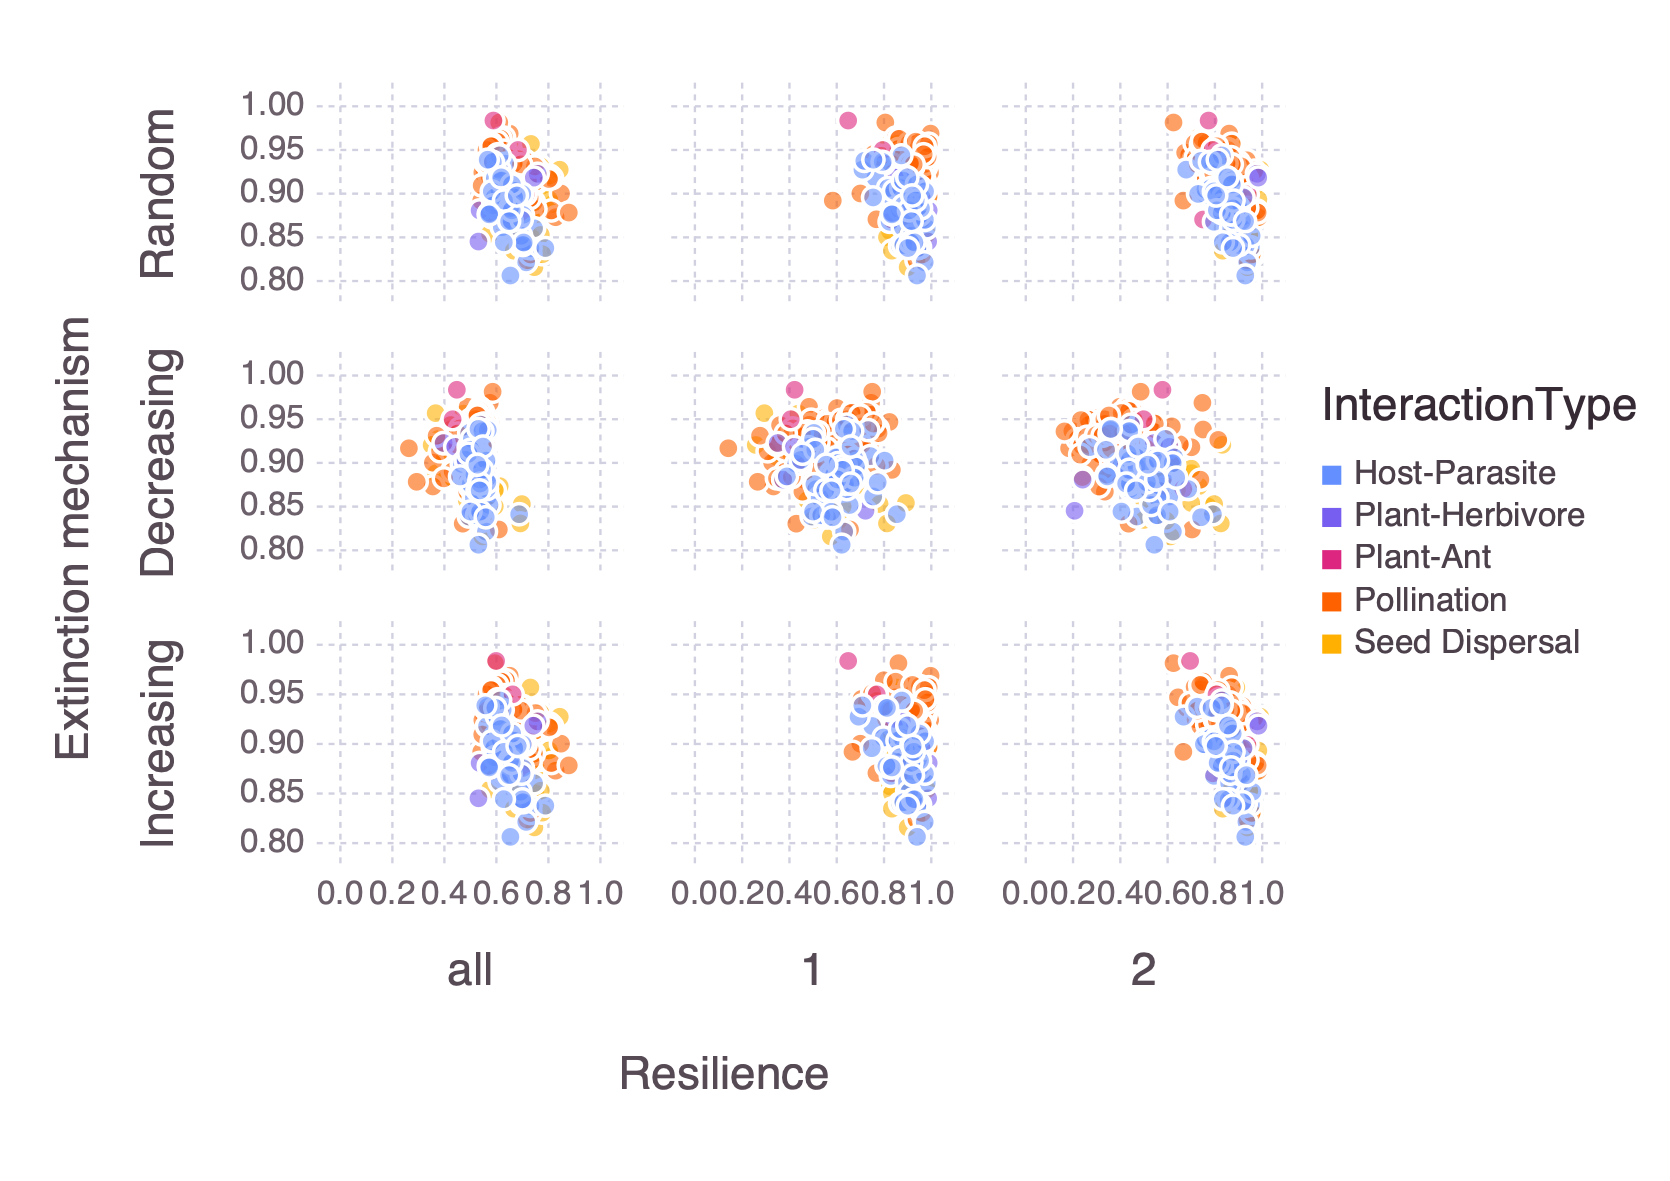
\includegraphics{figures/entropy_v_AUCall.png}
\caption{The relationship between SVD entropy and the area under an
extinction curve (as a proxy for resilience to extinction) for both
different extinction mechanisms (Random = the removal of a random
species, Decreasing = the removal of species in order of decreasing
number of interactions (i.e most to least number of interactions),
Increasing = the removal of species in order of increasing number of
interactions) as well as along different dimensions (species groups) of
the network (All = any species, Top-level = only top-level species, and
Bottom-level = only bottom- level species) Colours indicate the
different interaction types of the networks.}\label{fig:resilience}
}
\end{figure}

As highlighted in fig.~\ref{fig:other} SVD entropy can be used as an
additional measure of network complexity. However, as shown in
fig.~\ref{fig:resilience}, the assumption that network complexity begets
resilience to extinction begins to unravel when we use a measure of
physical complexity. This is in contrast to previous studies that have
shown how connectance plays a role in the resilience of networks to
extinctions (Dunne, Williams, and Martinez 2002; Memmott, Waser, and
Price 2004). This does not discount the role of using \emph{structural}
measures of network complexity (\emph{e.g.} connectance, nestedness or
spectreal radius) as indicators of their resilience (although possibly
hinting as to why there is no strong emerging consensus as to how
structural complexity relates to this), but rather points to an
erroneous assumption as to what aspects of a network we have previously
used to define its complexity.

\hypertarget{plant-pollinator-networks-are-slightly-more-complex}{%
\subsection{Plant-pollinator networks are slightly more
complex}\label{plant-pollinator-networks-are-slightly-more-complex}}

Although we don't observe clear differences in the relationship between
different interaction types when comparing amongst various measures of
complexity, we do find that different types of interaction networks have
differing SVD entropies. When comparing calculated SVD entropy between
interaction types using an ANOVA (after excluding Plant-Ant and
Plant-Herbivore interactions due to their small sample size in our
dataset) we find a significant difference between group means
(\(F = 47.047, p < 10^{-3}\)). A Tukey's HSD test reveals that
plant-pollinator networks (\(\mu = .924\)) are more complex than both
host- parasite networks (\(\mu = .885, p < 10^{-3}\)) and seed dispersal
(\(\mu = .888, p < 10^{-3}\)). Host-parasite and seed dispersal networks
had apparently no difference in average complexity (\(p = .889\)). These
results suggest that mutualistic networks may be more complex, which
matches with previous litterature: these networks have been shown to
minimise competition (Bastolla et al. 2009) and favour unique
interactions, thereby increasing network complexity. This specific
structure can appear as a side-process of either ecological (Maynard,
Serván, and Allesina 2018) or evolutionary (Valverde et al. 2018)
processes, but nevertheless leaves a profound imprint on the complexity
of the networks.

\begin{figure}
\hypertarget{fig:type}{%
\centering
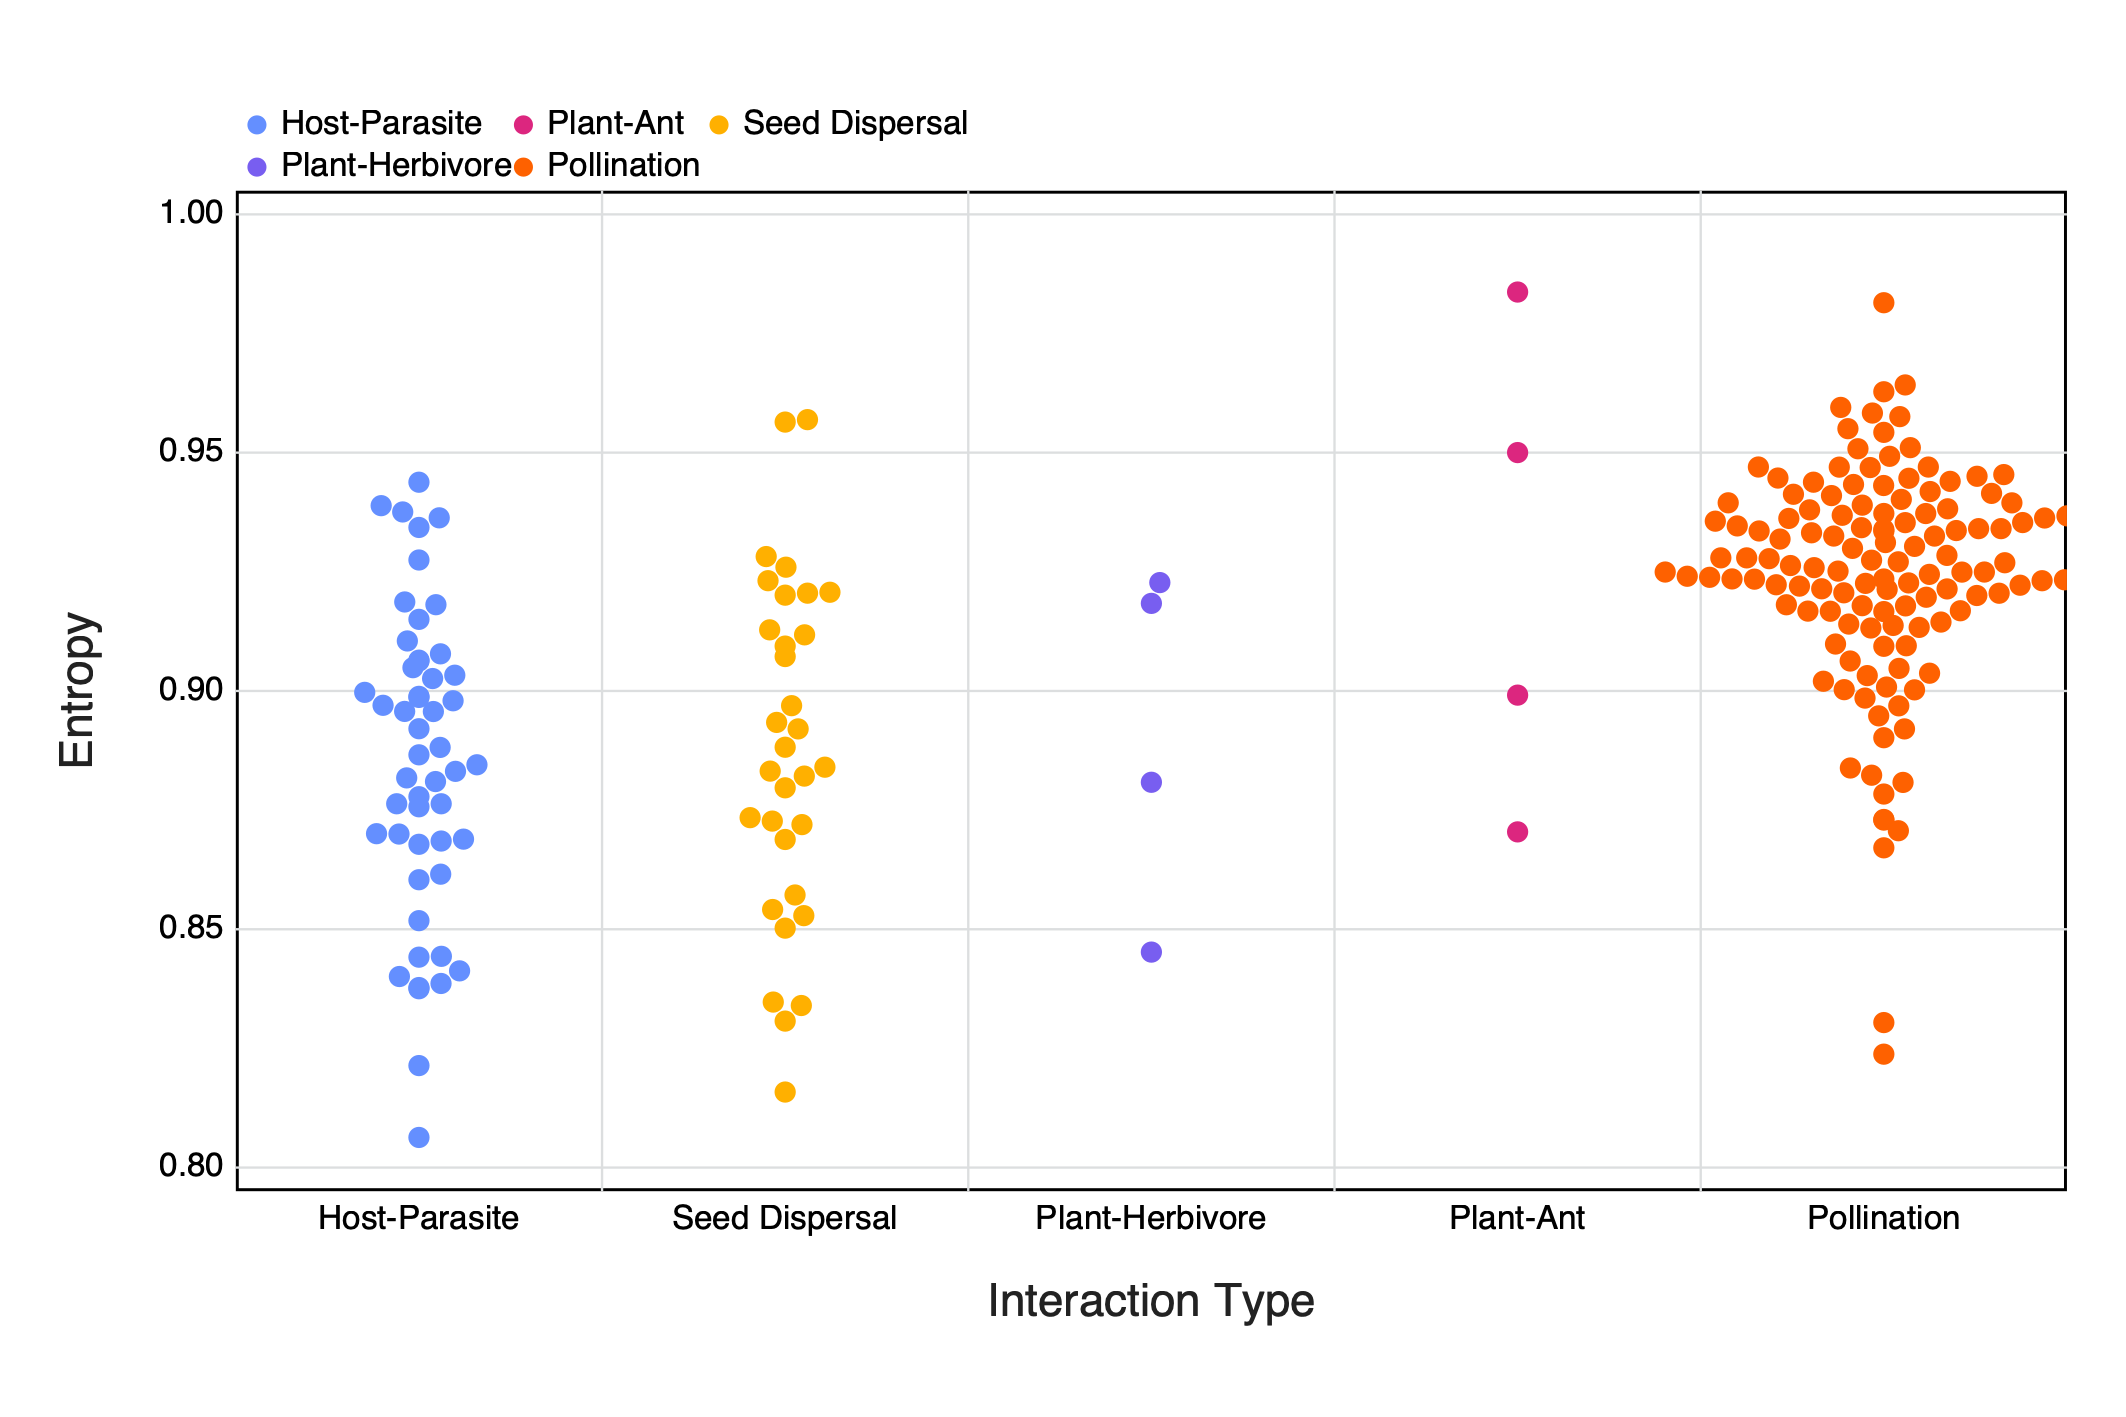
\includegraphics{figures/interactiontype_v_entropy.png}
\caption{The calculated SVD entropy of different interaction networks of
different interaction types}\label{fig:type}
}
\end{figure}

\hypertarget{connectance-constrains-complexity-but-also-rank-deficiency}{%
\subsection{Connectance constrains complexity (but also rank
deficiency)}\label{connectance-constrains-complexity-but-also-rank-deficiency}}

We used simulated annealing (Kirkpatrick 1984) to generate networks with
the highest, or lowest, possible SVD entropy values. From a set network
size (30 species, 15 on each side) with a random number of interactions
(spanning the entire range from minimally to maximally connected), we
reorganised interactions until the SVD entropy was as close to 0 or 1 as
possible. We repeated the process 25 times for every number of
interactions. We also measured the relative rank deficiency of the
generated networks. This allows identifying the boundaries of both
measures of complexity. The specific simulated annealing we used is as
follows. We set an initial temperature \(T_0 = 2\). At every timestep
\(t\) (up until \(t = 10^4\)), the temperature is set to
\(T_t = T_0\times\lambda^t\), so that is decays exponentially at a rate
\(\lambda = 1 - 10^{-4}\). At each timestep, we switch two interactions
in the network \(\mathcal{N}\) at random to generate a proposal network
\(\mathcal{M}\). The score of this proposal is the difference between
the squared error of \(\mathcal{N}\) and \(\mathcal{M}\) \emph{i.e.}
\(\Delta = (f(\mathcal{M})-\theta)^2-(f(\mathcal{N})-\theta)^2\), where
\(f\) is the SVD entropy and \(\theta\) is the target for optimisation
(either 0 or 1 for respectively minimally or maximally complex). A
proposal is accepted with probability
\(\text{P}(\mathcal{N} \rightarrow \mathcal{M} | \Delta) = \text{exp}\left(-\Delta\times T_t^{-1}\right)\).

By exploring the minimal and maximal values of SVD entropy for networks
of a given size, we can show that the range of complexity that a network
can express varies as a function of connectance (fig.~\ref{fig:simann}).
As reported by Poisot and Gravel (2014), there is no variation when the
networks are either minimally or maximally connected, but any
connectance in between can give rise to networks of varying
complexities. This being said -- minimally connected networks always
show the largest complexity, and an increase in connectance will always
decrease complexity. Interestingly, this relationship is monotonous, and
there is no peak of complexity where the maximal number of possible
networks combination exists, \emph{i.e.} around
\(\text{Co} \approx 0.5\) (Poisot and Gravel 2014). This is an
intriguing result -- ecological networks are indeed extremely complex,
but whereas ecologists have usually interpreted connectance as a measure
of complexity, it is in fact sparse networks that are the complex ones,
and connectance acts to decomplexify network structure.

\begin{figure}
\hypertarget{fig:simann}{%
\centering
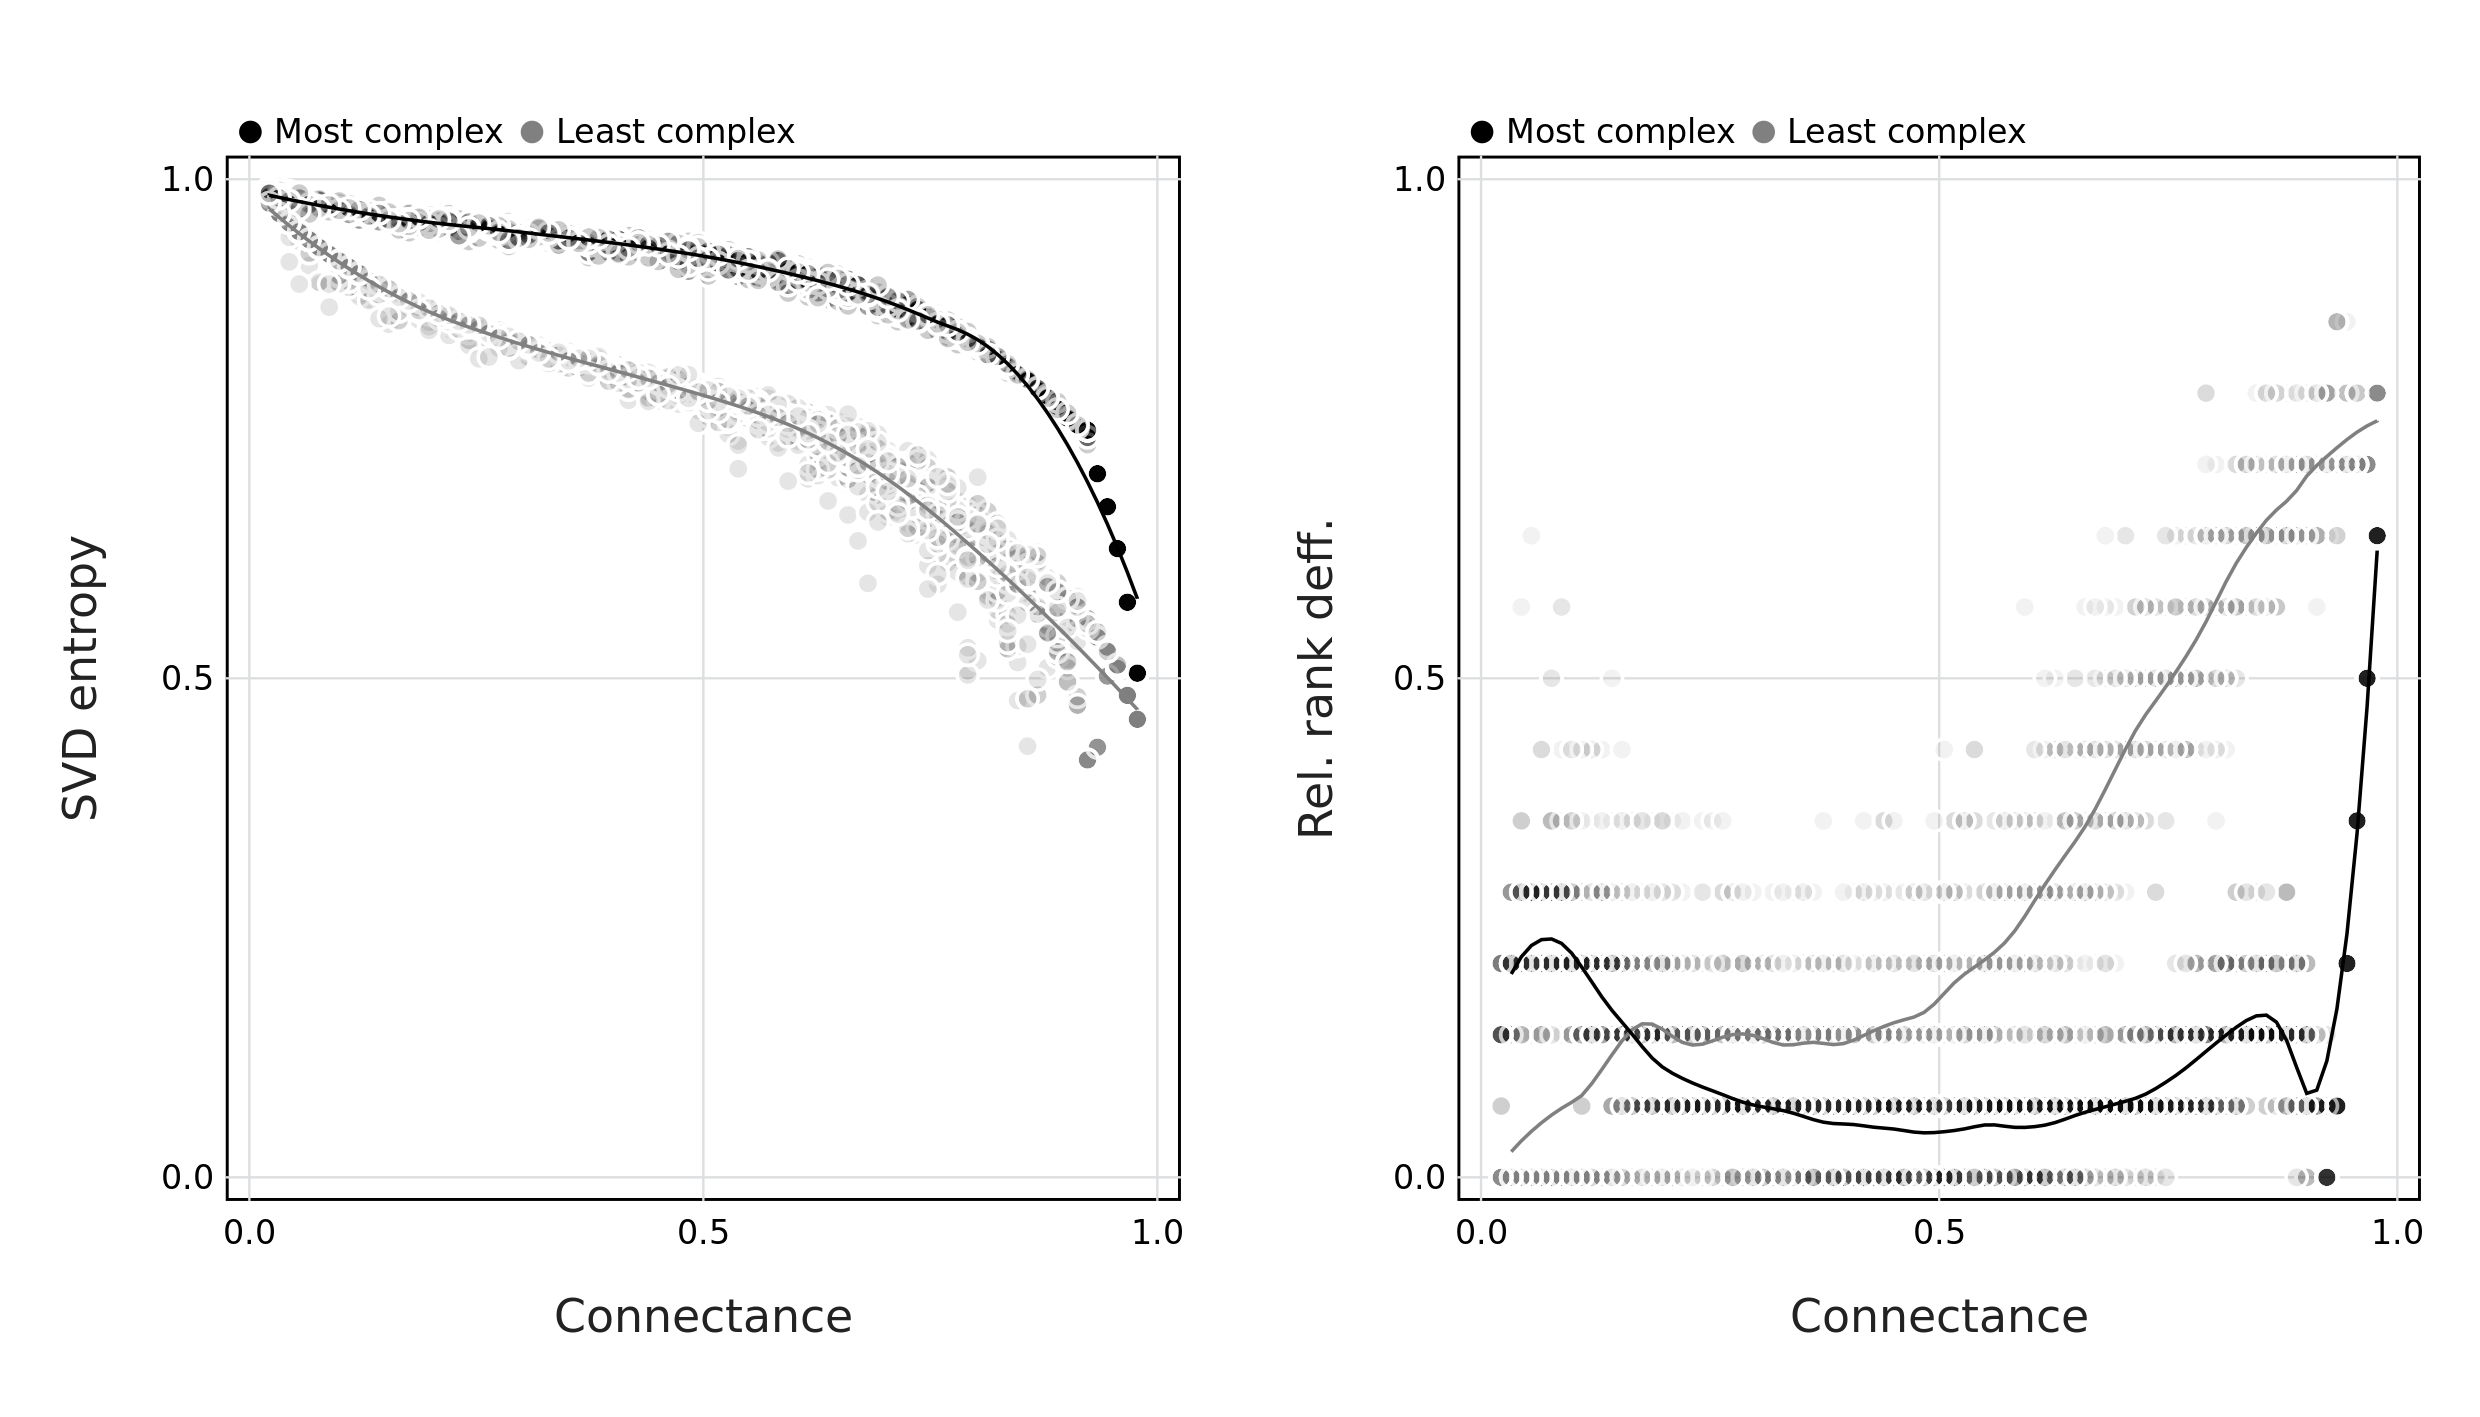
\includegraphics{figures/minmax_combined.png}
\caption{The relationship between the maximum and minimum value of SVD
entropy of a collection of random interaction networks (using simulated
annealing) for a given connectance spanning from 0 to 1 (left panel) and
how this relates to the relative rank deficiency of networks (right
panel)}\label{fig:simann}
}
\end{figure}

The right panel of fig.~\ref{fig:simann} shows the average rank
deficiency of networks for which SVD entropy was either maximised or
minimised. Complex networks (meaning, maximally complex given their
connectance) had a lower deficiency, indicating that except at extreme
connectances, there are combinations of networks for which all species
can interact in unique ways -- this is a natural consequence of the
results reported by Poisot and Gravel (2014), whereby the number of
possible networks is only really constrained at the far ends of the
connectance gradient. Minimally complex networks, on the other hand, saw
their rank deficiency increase with connectance. This hints at the fact
that the decrease in complexity with connectance may be primarily driven
by the infeasibility of having enough species for them to all interact
uniquely as connectance increases. Because non-unique interactions tend
to result in competition (Jordi Bascompte and Jordano 2007), this can
``push'' networks towards the full-rank configuration (as suggested by
the results in fig.~\ref{fig:size}), thereby maximising complexity
regardless of connectance.

\hypertarget{larger-networks-are-less-complex-than-they-could-be}{%
\subsection{Larger networks are less complex than they could
be}\label{larger-networks-are-less-complex-than-they-could-be}}

To assess whether ecological networks are more, or less, complex than
expected, we applied two null models that generate pseudo-random
networks: Type I (Fortuna and Bascompte 2006), where interactions happen
proportionally to connectance, and Type II (J. Bascompte et al. 2003),
where interactions happen proportionally to the joint degree of the two
species involved. The models are equivalent to, respectively, the
Erdos-Renyi and Configuration models (Newman 2010), both of which are
maximum entropy generative models that reflect global (Type I) or local
(Type II) constraints (Park and Newman 2004). We generated 999 samples
for every network in the dataset, and measured the \emph{z}-score of the
empirical network as

\begin{equation}\protect\hypertarget{eq:zscore}{}{z_i = \frac{x_i-\mu_i}{\sigma_i}}\label{eq:zscore}\end{equation}

where \(x_i\) is the SVD entropy of network \(i\), and \(\mu_i\) and
\(\sigma_i\) are respectively the average and standard deviation of the
distribution of SVD entropy under the null model. Negative values of
\(z_i\) reflect a network that has lower entropy than expected under the
assumptions of the null model. In fig.~\ref{fig:nullmod}, we show that
despite high \emph{absolute} values of SVD entropy, ecological networks
are not as complex as they \emph{could} be. This is consistently true
for both null models, and for the three types of networks that had a
sufficient sample size.

\begin{figure}
\hypertarget{fig:nullmod}{%
\centering
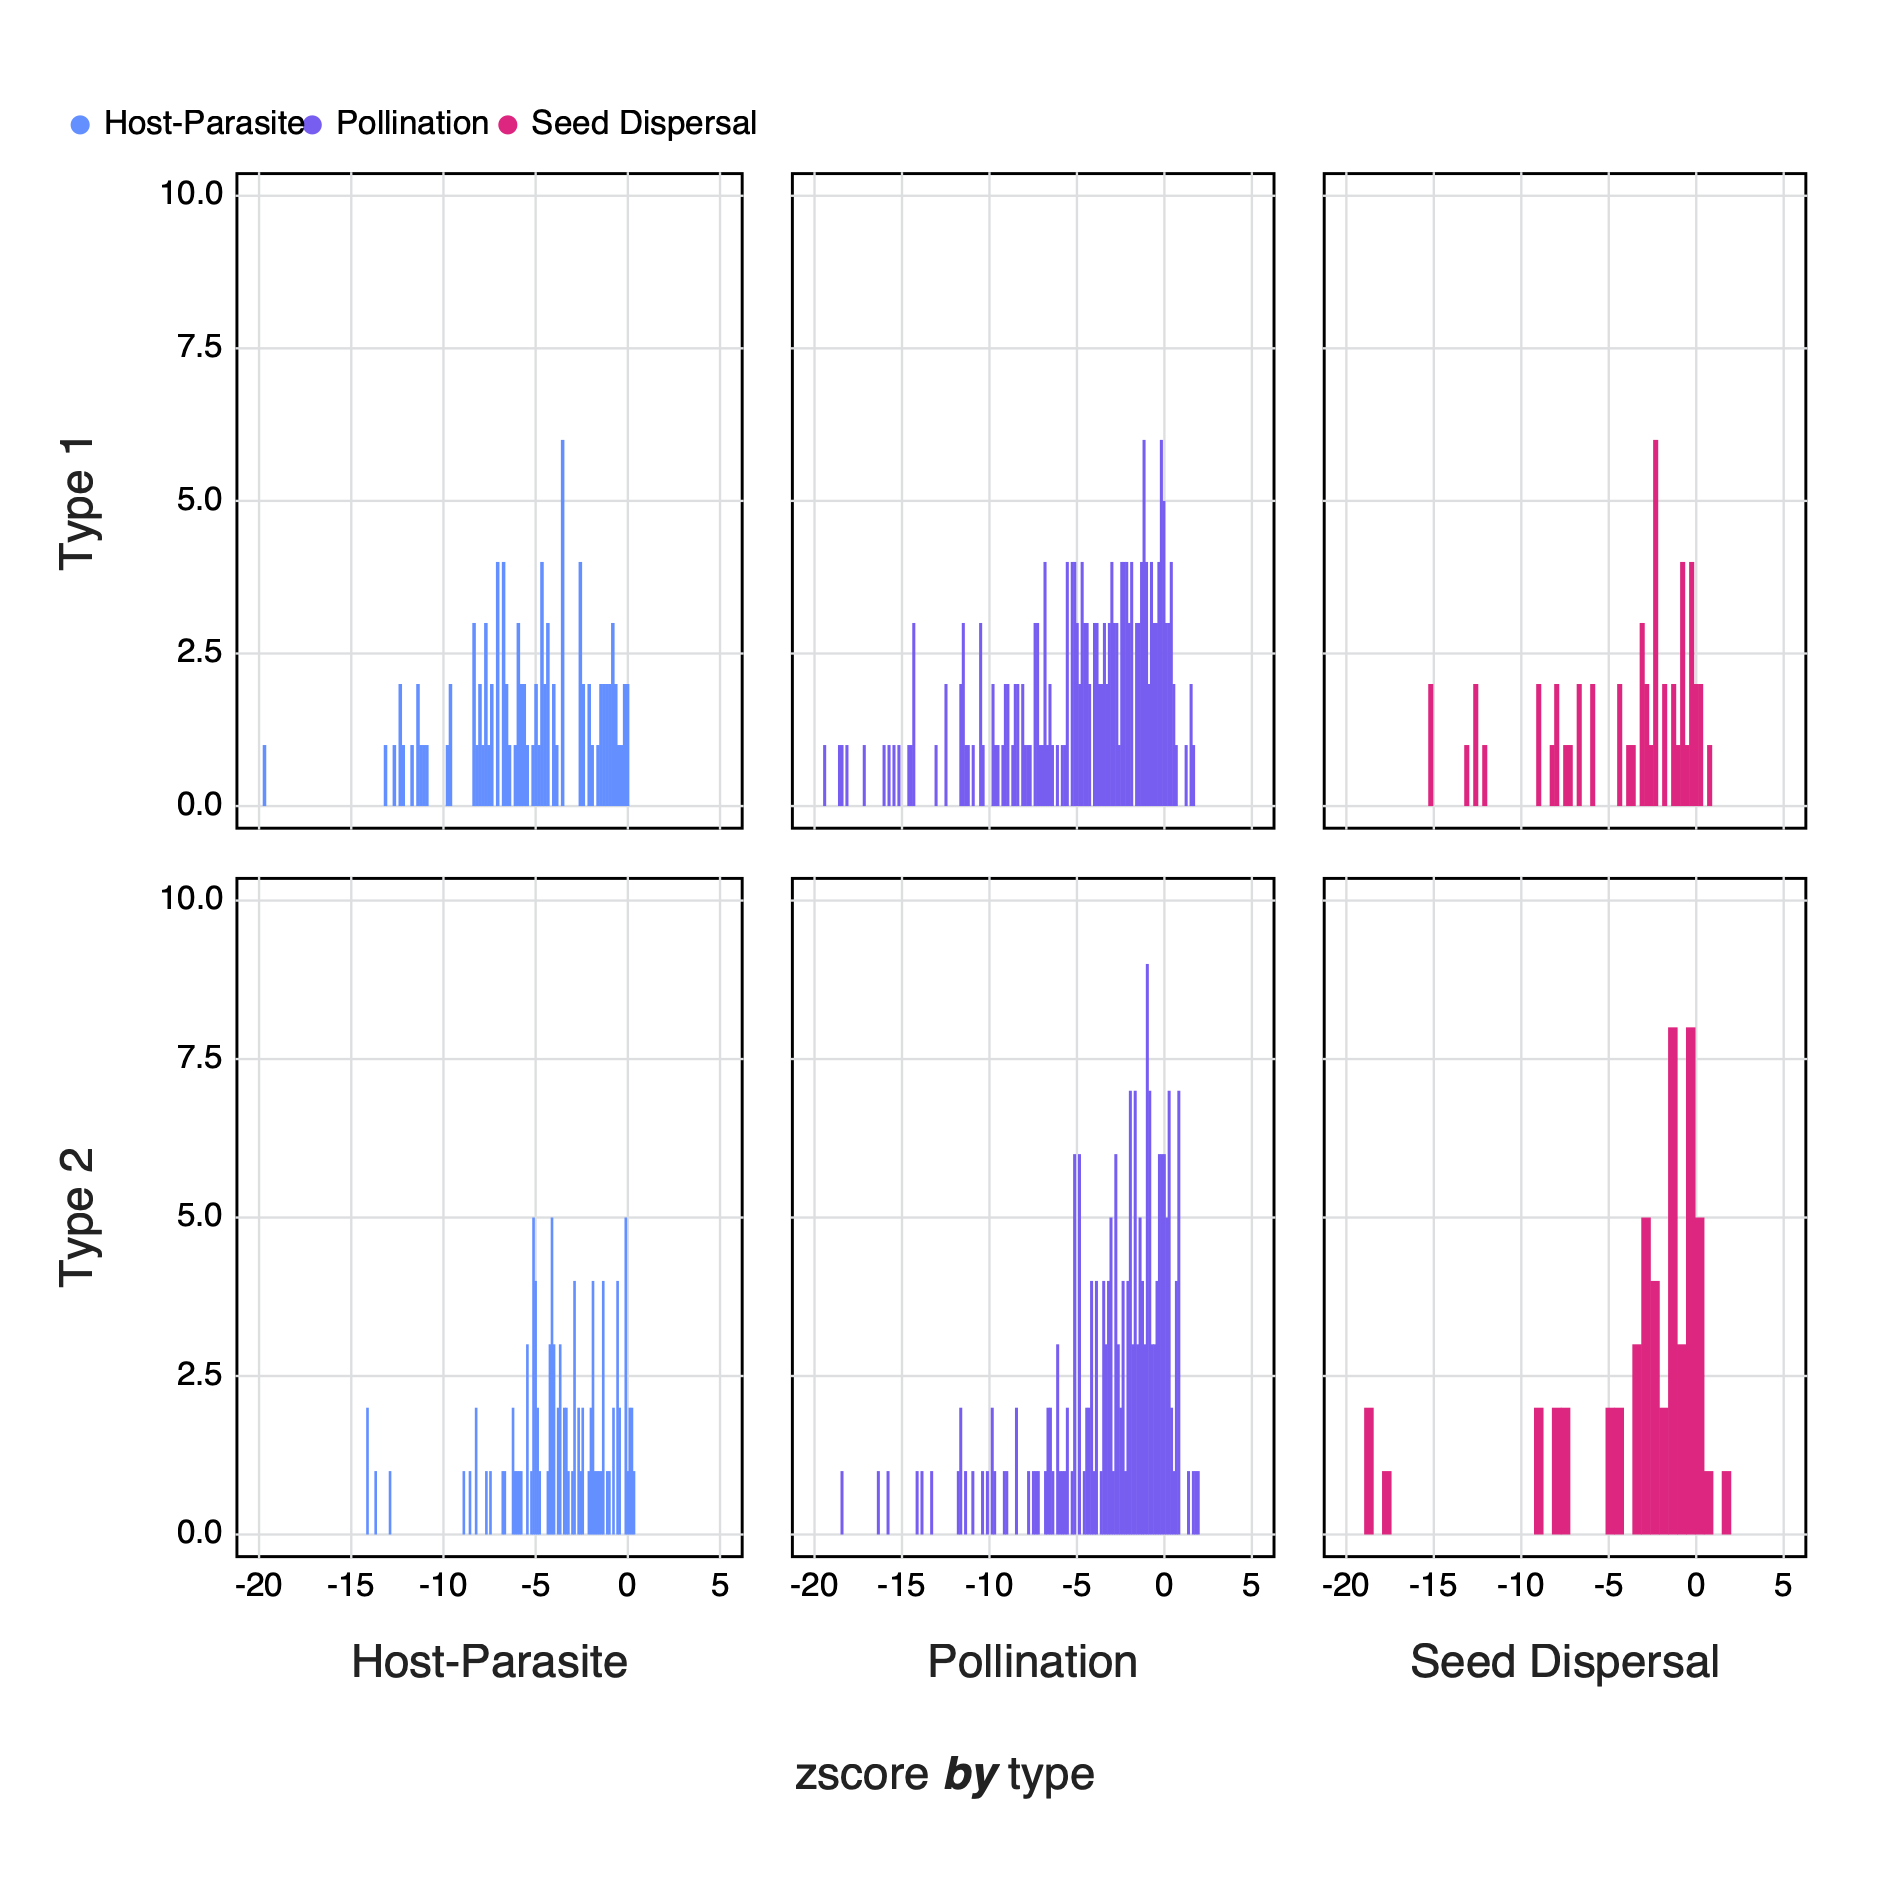
\includegraphics{figures/nullmodel_histogram.png}
\caption{The counts of the \(z_i\)-scores of different types of networks
for both Type I and Type II null models. Negative \(z_i\)-scores
indicate networks with an SVD entropy that is lower \emph{i.e.} less
complex than expected}\label{fig:nullmod}
}
\end{figure}

Previous work on random networks (using a model that is essentially the
Type I null model) shows that sufficiently large networks achieve
maximal von Neuman entropy (Du et al. 2010; Passerini and Severini
2011). In fig.~\ref{fig:larger}, we compare the \emph{logistic} of
\(z_i\) to the richness of the network. Transforming to the logistic
smooths out differences in absolute value that are apparent in
fig.~\ref{fig:nullmod}, and projects the values in the unit range, with
values above \(0.5\) being more complex than expected. It is quite
obvious that, across both models and the three types of interactions,
only smaller networks achieve higher entropy. Barbier et al. (2018) and
Saravia et al. (2018) have previously noted that the early stages of
network assembly usually result in severely constrained networks, due to
the conditions required for multiple species to persist; as networks
grow larger, these constraints may ``relax,'' leading in networks with
more redundancy, and therefore a lower complexity.

\begin{figure}
\hypertarget{fig:larger}{%
\centering
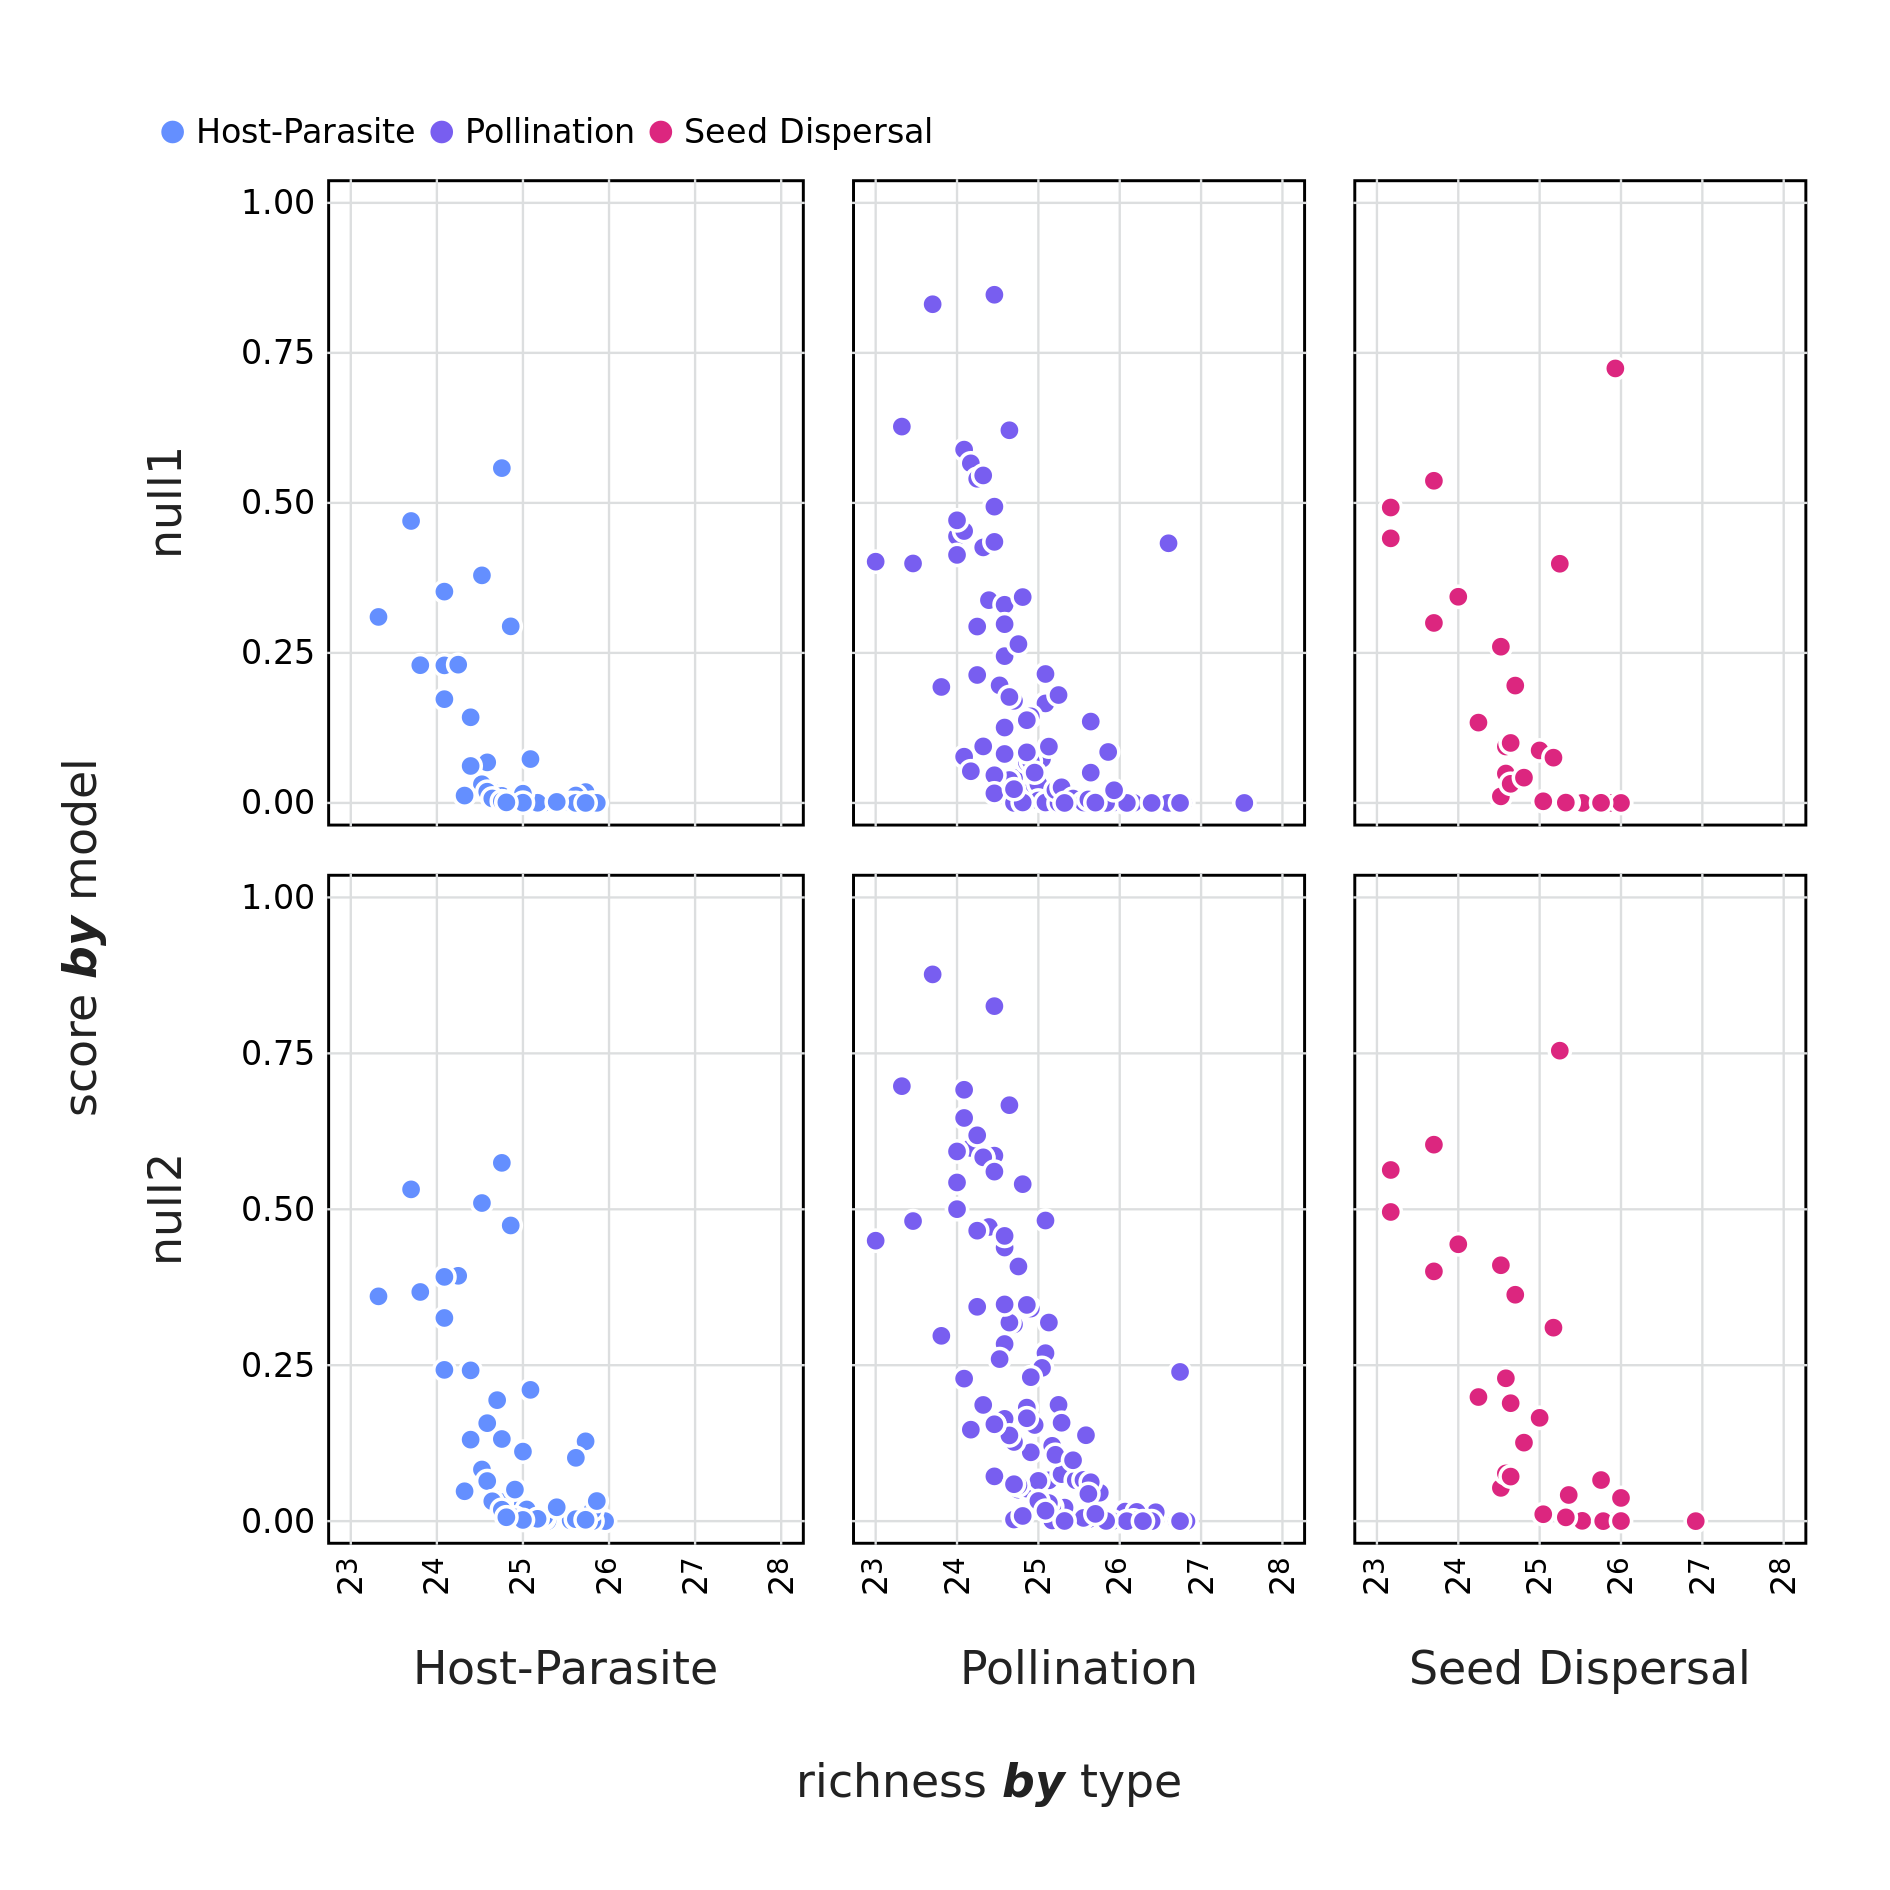
\includegraphics{figures/nullmodel_richness.png}
\caption{The logistic \(z_i\)-scores of different types of networks for
both Type I and Type II null models compared to the species richness of
the network. Where \(z_i\)-scores below 0.5 indicate networks with an
SVD entropy that is lower \emph{i.e.} less complex than
expected}\label{fig:larger}
}
\end{figure}

\hypertarget{conclusion}{%
\section{Conclusion}\label{conclusion}}

We present SVD entropy as a starting point to unifying (and
standardising) how we should approach defining the complexity of
ecological networks. The use of a unified definition will allow us to
revisit how complexity relates to the ecological properties of networks
using a standardised method. One important result from using SVD entropy
is that the complexity of ecological networks is indeed \emph{immense},
yet despite this high complexity networks are still not reaching their
\emph{maximum} potential complexity. We suggest that the assembly
dynamics of networks may explain this observation but this still raises
the question as to why larger (or more mature) networks are not
`maintaining' their expected complexity and prompts further exploration
as to the role of ecological assembly in structuring networks.

\hypertarget{references}{%
\section*{References}\label{references}}
\addcontentsline{toc}{section}{References}

\hypertarget{refs}{}
\begin{CSLReferences}{1}{0}
\leavevmode\hypertarget{ref-Adami2002WhaCom}{}%
Adami, Christoph. 2002. {``What Is Complexity?''} \emph{BioEssays} 24
(12): 1085--94. \url{https://doi.org/10.1002/bies.10192}.

\leavevmode\hypertarget{ref-Barbier2018GenAss}{}%
Barbier, Matthieu, Jean-François Arnoldi, Guy Bunin, and Michel Loreau.
2018. {``Generic Assembly Patterns in Complex Ecological Communities.''}
\emph{Proceedings of the National Academy of Sciences}, 201710352.
\url{https://doi.org/10.1073/pnas.1710352115}.

\leavevmode\hypertarget{ref-Bascompte2003NesAss}{}%
Bascompte, J., P. Jordano, C. J. Melian, and J. M. Olesen. 2003. {``The
Nested Assembly of Plant-Animal Mutualistic Networks.''}
\emph{Proceedings of the National Academy of Sciences} 100 (16):
9383--87. \url{https://doi.org/10.1073/pnas.1633576100}.

\leavevmode\hypertarget{ref-Bascompte2007PlaMut}{}%
Bascompte, Jordi, and Pedro Jordano. 2007. {``Plant-Animal Mutualistic
Networks: The Architecture of Biodiversity.''} \emph{Annual Review of
Ecology, Evolution, and Systematics} 38 (1): 567--93.
\url{https://doi.org/10.1146/annurev.ecolsys.38.091206.095818}.

\leavevmode\hypertarget{ref-Bastolla2009ArcMut}{}%
Bastolla, Ugo, Miguel A. Fortuna, Alberto Pascual-García, Antonio
Ferrera, Bartolo Luque, and Jordi Bascompte. 2009. {``The Architecture
of Mutualistic Networks Minimizes Competition and Increases
Biodiversity.''} \emph{Nature} 458 (7241): 1018--20.
\url{https://doi.org/10.1038/nature07950}.

\leavevmode\hypertarget{ref-Bezanson2017JulFre}{}%
Bezanson, J., A. Edelman, S. Karpinski, and V. Shah. 2017. {``Julia: A
Fresh Approach to Numerical Computing.''} \emph{SIAM Review} 59 (1):
65--98. \url{https://doi.org/10.1137/141000671}.

\leavevmode\hypertarget{ref-Borrelli2015SelIns}{}%
Borrelli, Jonathan J. 2015. {``Selection Against Instability: Stable
Subgraphs Are Most Frequent in Empirical Food Webs.''} \emph{Oikos} 124
(12): 1583--88. \url{https://doi.org/10.1111/oik.02176}.

\leavevmode\hypertarget{ref-Brose2006AllSca}{}%
Brose, Ulrich, Richard J. Williams, and Neo D. Martinez. 2006.
{``Allometric Scaling Enhances Stability in Complex Food Webs.''}
\emph{Ecology Letters} 9 (11): 1228--36.
\url{https://doi.org/10.1111/j.1461-0248.2006.00978.x}.

\leavevmode\hypertarget{ref-Delmas2018AnaEco}{}%
Delmas, Eva, Mathilde Besson, Marie-Hélène Brice, Laura A. Burkle,
Giulio V. Dalla Riva, Marie-Josée Fortin, Dominique Gravel, et al. 2018.
{``Analysing Ecological Networks of Species Interactions.''}
\emph{Biological Reviews}, 112540.
\url{https://doi.org/10.1111/brv.12433}.

\leavevmode\hypertarget{ref-Du2010NotNeu}{}%
Du, Wenxue, Xueliang Li, Yiyang Li, and Simone Severini. 2010. {``A Note
on the von Neumann Entropy of Random Graphs.''} \emph{Linear Algebra and
Its Applications} 433 (11): 1722--25.
\url{https://doi.org/10.1016/j.laa.2010.06.040}.

\leavevmode\hypertarget{ref-Duffy2007FunRol}{}%
Duffy, J. Emmett, Bradley J. Cardinale, Kristin E. France, Peter B.
McIntyre, Elisa Thébault, and Michel Loreau. 2007. {``The Functional
Role of Biodiversity in Ecosystems: Incorporating Trophic Complexity.''}
\emph{Ecology Letters} 10 (6): 522--38.
\url{https://doi.org/10.1111/j.1461-0248.2007.01037.x}.

\leavevmode\hypertarget{ref-Dunne2002NetStr}{}%
Dunne, Jennifer A., Richard J. Williams, and Neo D. Martinez. 2002.
{``Network Structure and Biodiversity Loss in Food Webs: Robustness
Increases with Connectance.''} \emph{Ecology Letters} 5 (4): 558--67.
\url{https://doi.org/10.1046/j.1461-0248.2002.00354.x}.

\leavevmode\hypertarget{ref-Eckart1936AppOne}{}%
Eckart, Carl, and Gale Young. 1936. {``The Approximation of One Matrix
by Another of Lower Rank.''} \emph{Psychometrika} 1 (3): 211--18.
\url{https://doi.org/10.1007/BF02288367}.

\leavevmode\hypertarget{ref-Forsythe1967ComSol}{}%
Forsythe, George, and Cleve Moler. 1967. \emph{Computer Solution of
Linear Algebraic Systems}. Englewood Cliffs, New Jersey: Prentice Hall.

\leavevmode\hypertarget{ref-Fortuna2006HabLos}{}%
Fortuna, Miguel A., and Jordi Bascompte. 2006. {``Habitat Loss and the
Structure of Plant-Animal Mutualistic Networks: Mutualistic Networks and
Habitat Loss.''} \emph{Ecology Letters} 9 (3): 281--86.
\url{https://doi.org/10.1111/j.1461-0248.2005.00868.x}.

\leavevmode\hypertarget{ref-Golub1987GenEck}{}%
Golub, G. H., Alan Hoffman, and G. W. Stewart. 1987. {``A Generalization
of the Eckart-Young-Mirsky Matrix Approximation Theorem.''} \emph{Linear
Algebra and Its Applications} 88-89: 317--27.
\url{https://doi.org/10.1016/0024-3795(87)90114-5}.

\leavevmode\hypertarget{ref-Golub1971SinVal}{}%
Golub, Gene H., and Christian Reinsch. 1971. {``Singular Value
Decomposition and Least Squares Solutions.''} In \emph{Linear Algebra},
134--51. Springer.

\leavevmode\hypertarget{ref-Gravel2016StaCom}{}%
Gravel, Dominique, François Massol, and Mathew A. Leibold. 2016.
{``Stability and Complexity in Model Meta-Ecosystems.''} \emph{Nature
Communications} 7: 12457. \url{https://doi.org/10.1038/ncomms12457}.

\leavevmode\hypertarget{ref-Gu2016HowLon}{}%
Gu, Rongbao, and Yanmin Shao. 2016. {``How Long the Singular Value
Decomposed Entropy Predicts the Stock Market? Evidence from the Dow
Jones Industrial Average Index.''} \emph{Physica A: Statistical
Mechanics and Its Applications} 453 (C): 150--61.

\leavevmode\hypertarget{ref-Jacquet2016NoCom}{}%
Jacquet, Claire, Charlotte Moritz, Lyne Morissette, Pierre Legagneux,
François Massol, Philippe Archambault, and Dominique Gravel. 2016. {``No
Complexitystability Relationship in Empirical Ecosystems.''}
\emph{Nature Communications} 7: 12573.
\url{https://doi.org/10.1038/ncomms12573}.

\leavevmode\hypertarget{ref-Kirkpatrick1984OptSim}{}%
Kirkpatrick, Scott. 1984. {``Optimization by Simulated Annealing:
Quantitative Studies.''} \emph{Journal of Statistical Physics} 34 (5-6):
975--86.

\leavevmode\hypertarget{ref-Landi2018ComSta}{}%
Landi, Pietro, Henintsoa O. Minoarivelo, Åke Brännström, Cang Hui, and
Ulf Dieckmann. 2018. {``Complexity and Stability of Ecological Networks:
A Review of the Theory.''} \emph{Population Ecology} 60 (4): 319--45.
\url{https://doi.org/10.1007/s10144-018-0628-3}.

\leavevmode\hypertarget{ref-Martinez1992ConCon}{}%
Martinez, Neo D. 1992. {``Constant Connectance in Community Food
Webs.''} \emph{The American Naturalist} 139 (6): 1208--18.

\leavevmode\hypertarget{ref-May1976SimMat}{}%
May, Robert M. 1976. {``Simple Mathematical Models with Very Complicated
Dynamics.''} \emph{Nature} 261 (5560): 459.
\url{https://doi.org/10.1038/261459a0}.

\leavevmode\hypertarget{ref-Maynard2018NetSpa}{}%
Maynard, Daniel S., Carlos A. Serván, and Stefano Allesina. 2018.
{``Network Spandrels Reflect Ecological Assembly.''} \emph{Ecology
Letters}, n/a--. \url{https://doi.org/10.1111/ele.12912}.

\leavevmode\hypertarget{ref-Memmott2004TolPol}{}%
Memmott, J., N. M. Waser, and M. V. Price. 2004. {``Tolerance of
Pollination Networks to Species Extinctions.''} \emph{Proceedings of the
Royal Society B: Biological Sciences} 271 (1557): 2605--11.
\url{https://doi.org/10.1098/rspb.2004.2909}.

\leavevmode\hypertarget{ref-Newman2010NetInt}{}%
Newman, Mark E. J. 2010. \emph{Networks. An Introduction}. New York, NY:
Oxford University Press.

\leavevmode\hypertarget{ref-Park2004StaMec}{}%
Park, Juyong, and M. E. J. Newman. 2004. {``Statistical Mechanics of
Networks.''} \emph{Physical Review E} 70 (6): 066117.
\url{https://doi.org/10.1103/PhysRevE.70.066117}.

\leavevmode\hypertarget{ref-Passerini2011NeuEnt}{}%
Passerini, Filippo, and Simone Severini. 2011. {``The von Neumann
Entropy of Networks.''} \emph{arXiv:0812.2597 {[}cond-Mat,
Physics:quant-Ph, q-Bio{]}}.
\url{https://doi.org/10.4018/978-1-60960-171-3.ch005}.

\leavevmode\hypertarget{ref-Phillips2011StrEco}{}%
Phillips, Jonathan D. 2011. {``The Structure of Ecological State
Transitions: Amplification, Synchronization, and Constraints in
Responses to Environmental Change.''} \emph{Ecological Complexity},
Special section: Complexity of Coupled Human and Natural Systems, 8 (4):
336--46. \url{https://doi.org/10.1016/j.ecocom.2011.07.004}.

\leavevmode\hypertarget{ref-Pielou1975EcoDiv}{}%
Pielou, E. C. 1975. \emph{Ecological Diversity}. New York: Wiley.

\leavevmode\hypertarget{ref-Poisot2019EcoJl}{}%
Poisot, Timothée, Zacharie Belisle, Laura Hoebeke, Michiel Stock, and
Piotr Szefer. 2019. {``EcologicalNetworks.jl - Analysing Ecological
Networks.''} \emph{Ecography}. \url{https://doi.org/10.1111/ecog.04310}.

\leavevmode\hypertarget{ref-Poisot2014WheEco}{}%
Poisot, Timothée, and Dominique Gravel. 2014. {``When Is an Ecological
Network Complex? Connectance Drives Degree Distribution and Emerging
Network Properties.''} \emph{PeerJ} 2: e251.
\url{https://doi.org/10.7717/peerj.251}.

\leavevmode\hypertarget{ref-Poulin2010NetAna}{}%
Poulin, Robert. 2010. {``Network Analysis Shining Light on Parasite
Ecology and Diversity.''} \emph{Trends in Parasitology} 26 (10):
492--98. \url{https://doi.org/10.1016/j.pt.2010.05.008}.

\leavevmode\hypertarget{ref-Proulx2005NetThi}{}%
Proulx, Stephen R., Daniel E. L. Promislow, and Patrick C. Phillips.
2005. {``Network Thinking in Ecology and Evolution.''} \emph{Trends in
Ecology \& Evolution} 20 (6): 345--53.
\url{https://doi.org/10.1016/j.tree.2005.04.004}.

\leavevmode\hypertarget{ref-Rozdilsky2001ComCan}{}%
Rozdilsky, Ian D., and Lewi Stone. 2001. {``Complexity Can Enhance
Stability in Competitive Systems.''} \emph{Ecology Letters} 4 (5):
397--400. \url{https://doi.org/10.1046/j.1461-0248.2001.00249.x}.

\leavevmode\hypertarget{ref-Saravia2018EcoNet}{}%
Saravia, Leonardo A., Tomas Ignacio Marina, Marleen De Troch, and
Fernando R. Momo. 2018. {``Ecological Network Assembly: How the Regional
Meta Web Influence Local Food Webs.''} \emph{bioRxiv}, 340430.
\url{https://doi.org/10.1101/340430}.

\leavevmode\hypertarget{ref-Shannon1948MatThe}{}%
Shannon, C. E. 1948. {``A Mathematical Theory of Communication.''}
\emph{The Bell System Technical Journal} 27 (3): 379--423.
\url{https://doi.org/10.1002/j.1538-7305.1948.tb01338.x}.

\leavevmode\hypertarget{ref-Staniczenko2013GhoNes}{}%
Staniczenko, Phillip P. A., Jason C. Kopp, and Stefano Allesina. 2013.
{``The Ghost of Nestedness in Ecological Networks.''} \emph{Nature
Communications} 4 (1): 1391. \url{https://doi.org/10.1038/ncomms2422}.

\leavevmode\hypertarget{ref-Ulrich2009ConSG}{}%
Ulrich, Werner, Mário Almeida-Neto, and Nicholas J. Gotelli. 2009. {``A
Consumer's Guide to Nestedness Analysis.''} \emph{Oikos} 118 (1): 3--17.

\leavevmode\hypertarget{ref-Valverde2018ArcMut}{}%
Valverde, Sergi, Jordi Piñero, Bernat Corominas-Murtra, Jose Montoya,
Lucas Joppa, and Ricard Solé. 2018. {``The Architecture of Mutualistic
Networks as an Evolutionary Spandrel.''} \emph{Nature Ecology \&
Evolution} 2 (1): 94. \url{https://doi.org/10.1038/s41559-017-0383-4}.

\end{CSLReferences}

\end{document}
